\documentclass[onecolumn,11pt,preprint]{sigplanconf}

% \documentclass{llncs}
% \documentclass{article}

\usepackage{amsmath}
\usepackage{times}
\usepackage{comment}
\usepackage{url}
\usepackage{fancyvrb}
\usepackage{graphics}
\usepackage{boxedminipage}
\usepackage{code}

\usepackage[bookmarks=false,%
            colorlinks,linkcolor=black,urlcolor=blue,%
            pdfauthor={Oleg and Keean and Ralf},%
            pdftitle={OOHaskell}]{hyperref}


\DefineShortVerb{\|}
%\DefineVerbatimEnvironment{code}{Verbatim}{xleftmargin=\mathindent,commandchars=\\\{\},fontsize=\small}
% \setlength{\parskip}{0pt}
%\newlength{\mathindent}
%\setlength{\mathindent}{1em}


% Macros for notes to each other in the text
\newcommand{\keean}[1]{{\it [Keean says: #1]}}
\newcommand{\oleg}[1]{{\it [Oleg says: #1]}}
\newcommand{\ralf}[1]{{\it [Ralf says: #1]}}

\newcommand{\mysize}{\small}
\newcommand{\myskip}{\smallskip}
\newcommand{\antiskip}{\vspace{-25\in}}
\newcommand{\myinput}[1]{The content of this section is not yet released.}
\newcommand{\HList}{\textsc{HList}}
\newcommand{\undefined}{\ensuremath{\bot}}
\newcommand{\Forall}{\ensuremath{\forall}}

\setlength{\parskip}{0pt}
\setlength{\parsep}{0pt}
 


\begin{document}

%\conferenceinfo{WXYZ '05}{date, City.} 
%\copyrightyear{2005} 
%\copyrightdata{supplied by printer} 
 
\title{Haskell's overlooked object system\\
{\small ---~DRAFT OF \today~---}\vspace{-77\in}}

\authorinfo{Oleg Kiselyov}{FNMO Center, Monterey, CA}{}
\authorinfo{Ralf L{\"a}mmel}{Microsoft Corp., Redmond, WA}{}
\authorinfo{Keean Schupke}{Imperial College, London, UK}{}


\maketitle

\begin{abstract}

Haskell provides type-class-based bounded polymorphism as opposed to
subtype polymorphism of object-oriented languages such as Java and
OCaml. It is a contentious question whether Haskell (alone or with
extensions) can support conventional object-oriented programming with
encapsulation, inheritance, overriding, statically checked subtyping,
and so on.

\medskip

Recently it has been shown that multi-parameter type classes with
functional dependencies alone support the record calculus for
extensible polymorphic records with first-class labels and
subtyping. This paper builds upon this result and shows that Haskell
readily supports objects encapsulating methods and mutable fields,
inheritance, overriding, constructor methods, abstract classes,
lexically scoped classes, in fact, first-class classes, and others. We
provide open recursion, and the ability to close it selectively, thus
giving the programmer full control over sharing or isolation of base
classes in multiple-inheritance hierarchies. It is especially pleasing
that the class instantiator is just the (monadic) fix-point
combinator.

\medskip

We work through a series of working OO examples as they are commonly
found in OO textbooks and programming language tutorials. In
particular, we elucidate a translation of OCaml's object syntax to
Haskell, where we do not perturb the OCaml code: we translate
expression-by-expression without a need for global parameters. More
generally, we aim to provide OO idioms in Haskell in an OO
intuition-preserving way. The resulting combination of OO idioms,
higher-order functional programming, and type inference is
comparatively powerful. Hence, `OOHaskell' lends itself as a prime
environment for typed OO language design.

\end{abstract}

\makeatactive



%%%%%%%%%%%%%%%%%%%%%%%%%%%%%%%%%%%%%%%%%%%%%%%%%%%%%%%%%%%%%%%%%%%%%%%%%%%%%
%%%%%%%%%%%%%%%%%%%%%%%%%%%%%%%%%%%%%%%%%%%%%%%%%%%%%%%%%%%%%%%%%%%%%%%%%%%%%
%%%%%%%%%%%%%%%%%%%%%%%%%%%%%%%%%%%%%%%%%%%%%%%%%%%%%%%%%%%%%%%%%%%%%%%%%%%%%



\section{Before Intro}

We must address relavance and significance: for practioneers, for
the programming language design, and for theory.

The issue of OO and Haskell, OO classes vs. type classes shows up on
Haskell mailing lists and websites with remarkable regularity.
[
the latest ones
\url{http://www.haskell.org//pipermail/haskell/2004-June/014164.html}
\url{http://www.haskell.org/tmrwiki/LearningHaskellNotes#head-f9911730c98633f6182b33ce159a77d72afc6d87}
]

One can't deny deep interest in this subject. The range of approaches and
differences in opinion (see summaries in \cite{MonadReader3} as well as
LearningHaskellNotes above) show that the question is unsettled one.
The often repeated advice is that we can't do the ``classical'' OO in
Haskell. If we wish for OO, it has to be done in a totally different
(not often obvious: Message on Haskel-Cafe, form Alistair
Bayley) way. If we wish to approach the classical OO of Java, C++,
or of Javascript, etc., extensions to Haskell are needed. Such
extensions have indeed been proposed, with the motivation of ...

One of the main motivations, stated in \cite{MonadReader3} is to be able to
bring OO programmers into Haskell fold, or to be able to port existing
OO code to Haskell without totally rewriting it.  ``That said, it
might be that you need to interface with external OO code, or you are
porting an existing program and need to remain faithful to the
original design, if only because you don't understand it well enough
to convert it to a functional design.'' \cite{MonadReader3}.


There is an intellectual challenge as well, of seeing if the
conventional OO can at all be implemented in Haskell. The paper on
imperative programming in Haskell \cite{peytonjoneswadler-popl93}
epitomizes this approach. We should also mention FC++ \cite{fcpp-jfp},
which attempted to see if Haskell Prelude can be implemented in
C++. Clearly it is the (possibility) of a faithful translation rather the
end result of it that is the motivation.

The present paper follows the same intellectual tradition: can we
faithfully implement X in Y (specifically excluding writing of the
compiler for X in Y. Make this a footnote?)? Or, if X is expressible
\cite{Felleisen90} in Y?  For one thing, we settle the question: the
conventional OO is expressible in current Haskell without any new
extensions. It turns out, Haskell98 plus multi-parameter type classes
with functional dependencies are enough. Even overlapping instances
are not essential (yet using them permits a more convenient
representation of labels).  That conclusion has not been known
before\footnote{ Haskell is not even supposed to have extensible
  polymorphic records! At least that was the general belief until a
  few months ago.  There were many debates on the Haskell mailing list
  about adding such records to Haskell. At the Haskell 2003
  workshop~\cite{HW03}, this issue was selected as prime topic for
  discussion.}; and, as being emphasized by many people and reviewers,
is novel and surprising.

Our encoding of objects in this paper is deliberately conventional.
Our goal is not to find some new way to encode objects; rather, find a
way to realize the traditional object encoding based on record
subtyping. One of the main goals of this paper is to be able represent
the conventional OO code, in as straightforward way as possible.
We wish to satisfy the real practical need expressed in
\cite{MonadReader3}, that is [port code without undue mangling -- w/o
  global transformation].

For the sake of simplicity, our object encoding is simple, based on
`flat' extensible records with subtyping. More efficient
representation based on method table and field table is left for
another paper. Although our current encoding is certainly not
optimal, it is conceptually clearer. Furthermore, it is close to the
object encoding used in such languages as Perl, Python, Lua, and thus
helps in an earlier stated goal (correlating mainstream OO with
Haskell).  The encoding is often the first one to be used when adding
OO to the existing language -- and thus seems to be suitable starting
point for us.  Again, for clarity and for easy correlation with
practice, we will be concerend with mutable objects (implemented via
|IORef| or |STRef|). Most OO system in
practical use have mutable state. Functional objects bring quite
an interesting twist and so will be considered in another paper.

From one angle, the present paper can be considered an `inverse' of
FC++. The latter tried to implement in C++ the quintessentials Haskell
features: type inference, higher-order, non-strictness. The present
paper illustrates faithful (to be more precise, in similar syntax and
without requiring global program transformation) representation of one
of the important C++ feature: OO. Section XXX discusses one of the
popular benchmarks -- Shapes. 


One may be tempted to dismiss the paper as ``just type hacking''. We
defend both on the practical grounds, language design grounds, and the
theoretical grounds \footnote{Multi-parameter type classes with
  functional dependencies are \emph{not} a hack: they are
  well-formalized and reasonably understood~\cite{SS04}.}. From the
practical point of view: the fact that we found a quite unexpected
(and unintended) use of a particular language feature does not mean
that the result is practically useless. Template meta-programming in
C++ has been the best known example of such ``type hacking''. And yet
it has lead to |boost|, which has become a de facto tool for modern
C++ programming (Adobe uses Boost:
\url{http://lambda-the-ultimate.org/node/view/563#comment-4531}).
Templates and template meta-programming have changed the very
character of the language (\cite{fcpp-jfp})
[Stroustrup interview? Need some reference. If we
  can't find any, I can use LtU references
\url{http://lambda-the-ultimate.org/node/view/663}
(see comments by Scott Johnson)
\url{http://lambda-the-ultimate.org/node/view/663#comment-5839}
See also:
\url{http://spirit.sourceforge.net/distrib/spirit_1_7_0/libs/spirit/phoenix/doc/preface.html}
] and made generative
research and practice in C++ possible (\cite{DSL-in-three-lang}).

Just as C++ has become the laboratory for generative programming
\cite{DSL-in-three-lang} and lead to such applications as FC++, we contend
that Haskell can become the laboratory for OO design and development.
To extend the motto by Simon Peyton-Jones, Haskell is not only the
best imperative language. It is the best OO language as well.
C++ programmers now routinely use parsing combinators, thanks to the
|boost::spirit| library. Haskell programmers can likewise use OO idioms if it
suits the problem at hand. We can experiment with OO features and gain
experience, without the need to change Haskell compilers.

We shall point out in Sections XXX and XXX (simple objects?),
OOHaskell already exhibits features that are either bleading-edge or
unattainable in mainstream OO languages: for example, first-class
classes and class closures; statically typechecked collection classes
with bounded polymorphism of collection arguments; multiple
inheritance with user-controlled sharing. It is especially remarkable
that these and more familiar object-oriented features are not
introduced by fiat -- we get them for free. For example, the type of a
collection with bounded polymorphism of elements is inferred
automatically by the compiler. Abstract classes cannot be instantiated
not because we say so but because the program will not typecheck
otherwise.  \oleg{Mention more ``major byproducts'' from the sections
  below} We have experienced first-hand the incredible amount of
guidance Haskell type system gives in the design of OO features.

We should not overlook a theoretical contribution. On one hand, it is
indeed well-known that we can build OO systems on top of extensible
records (introduced earlier in the HList paper) with a suitable notion
of subtyping \cite{Cardelli-on-understanding}. Also, an
object-oriented system with `flat' mutable objects is significantly
simpler theoretically; one may think that none of the machinery
[Pierce] of existential or recursive types is needed. We must point
out that even mutable objects implemented on the top of extensible
records are more complex than it may appear. The complexity comes from
supporting inheritance and virtual methods. Even in the case of flat
mutable objects (records of closures), the typing of `self' presents
challenges (seem to require recursive type -- lift phrases from
subsection ``{OOHaskell~---~A challenge}'' below). Furthermore, to implement
a homogeneous list of objects all supporting the same interface (Shape
example), one seem to need existential types. Both recursive types and
existential make inference impossible, in current Haskell. The user
must give explicit type annotations. In the paper we show that we
support open recursion, virtual methods, and homogeneous lists of
diferently implemented Shapes without resorting to recursive object
types and to existentials. Therefore, the object types can be
\emph{inferred}.

Another theoretical problem -- even with mutable objects -- is the
controversy regarding covariance and contravariance of method
arguments \cite{SG04}, \cite{catcall}. Our work shows how to implement
covariant methods (which are considered practically desirable [Eiffel
  FAQ]) and statically (at compile-time) maintain soundness. Alas, due
to the lack of space, we merely skim the topic and refer the reader to
the code (and the next paper).


List all the suboptimal OO encoding, with refs,
and discuss their drawbacks (including earlier Shape examples).
Mention that there are simpler solutions, but they all fall short of
the complete OO encoding. This paper seems to be the one that treats
OO in full generality, including open recursion, interface and
implementation inheritance, subtyping.

A reviewer wrote:
``The encoding is quite simple --- it's surprising that
everything is so easy --- yet not at all obvious. The paper isn't
labelled as a pearl, but would certainly fit well in that category.''

A reviewer wrote:
``The result might seem poor and just containing clever tricks
however it took 10 years to obtain that proof of concepts and this
deserves attention.''


We must mention two other issues: error messages and efficiency of
encoding.

One may think that the inferred types and error messages
would be nearly incomrehensible. That is not actually the case.
We give an example of the inferred type, in Section (about Selfish
types). The type of the constructor, for example, 
essentially lists all the fields of an object, both new and
inherited. The error messages (e.g., from an attempt to instantiate
|abstract_point|, in the same section) succinctly list just the
missing field. In general, the clarity of error messages is undoubtably
is an area that needs more research, and more research is
being done (Sulzmann), which we or compiler writers may take advantage
of. It must be mentioned that error messages in C++ (template
instantiation) can be immensely
verbose, spanning literally 30 and 40 packed lines. And yet boost and
similar libraries that extensively use templates are gaining momentum.

Another issue is the efficiency of the encoding.  In the present
paper, we specifically post-poned any optimizations for the sake of
conceptual clarity.  For example, although record extension is
constant (run-)time, the field/method lookup is linear search. Clearly
a more efficient encoding is possible: one reprentation of the labels
in the \HList\ paper permits the total order among the labels (and label
types! they are singleton types), which in turn, permits construction
of efficient search trees. In this first OOHaskell paper, we chose the
conceptual clarity over such optimizations.


``For these reasons, the method is likely to be of limited value in
practice, unless Haskell compilers start providing special support for
the encoding itself. But showing the usefulness of such an encoding is
the first step towards encouraging compiler writers to do so!''




Todo: 
\begin{enumerate}
\item ``The power of the system is first proved by encoding some very basic
examples from the ocaml tutorial. For this part, page 6 gives the basic
encoding, but pages 7 to 9 just repeat this basic encoding, with no
new information.''
So, drop pages 7-9?
\end{enumerate}

% http://dblp.uni-trier.de


\section{Introduction}

\oleg{Explicitly enumerate the contributions.}

\subsection*{OOP and Haskell~---~Married finally}
\oleg{move this subsection up?}
There is a widely shared perception regarding the relation between
Haskell and object-oriented programming (OOP). That is, Haskell is
thought to really lack OOP essentials. The functionally minded OOP
aficionado could either wish for an extended Haskell, employ a
multi-language setup such as .NET, or disregard Haskell and go for
OCaml instead, which is known to be a mainstream functional
programming language that provides an advanced OOP system. This
perception is without basis. In this paper, we show how to program
with mutable objects, inheritance, subtyping etc.\ \emph{in Haskell}
using only common type-system extensions. More than that, we will end
up with a comparatively rich combination of OO idioms, higher-order
functional programming, and type inference. We therefore think that
(OO)Haskell lends itself as environment for advanced and typed OO
\emph{language design}. We will illustrate OOHaskell with a series of
practical examples as they are commonly found in OO textbooks and
programming language tutorials. We wish to make OOHaskell as easy as
possible to use by an experienced OO programmer who is migrating to
Haskell. We certainly could emulate the OO system of OCaml or Java by
writing a compiler in Haskell for these languages. But that's not the
sort of emulation we aim at. We wish our OOHaskell system to be just
as expressive~\cite{Felleisen90} as the most advanced OO
systems. Informally, we wish our OO code looked `just the same as
native OO code'~---~or perhaps even better, with less syntactic sugar.


\subsection*{OOHaskell~---~A challenge}

We will marry Haskell and OO by going through the following sequence:
extensible polymorphic records, record calculus, objects with mutable
data, classes with subtyping, open recursion, inheritance,
polymorphism. That sounds quite simple until we realise that, for one
thing, Haskell is not even supposed to have extensible polymorphic
records. At least that was the general belief until a few months ago.
There were many debates on the Haskell mailing list about adding such
records to Haskell. At the Haskell 2003 workshop~\cite{HW03}, this
issue was selected as prime topic for discussion. Fortunately, this
problem is resolved. In our very recent work on strongly typed
heterogeneous collections~\cite{HLIST-HW04}, we have provided
collection types such as extensible records using Haskell's type
classes.

There is a second major barrier for OOHaskell: the notion of
`self'. That is, the realisation of objects with inheritance and
polymorphism in terms of records seems to require (equi-) recursive
types, to type `self'~\cite{PT94}.
%
% See p. 29 of the paper and the quotation from Bruce, 1992. Pierce
% seems to agree that recursive types are needed to model inheritance
% of methods involving self. -- beginning of the second paragraph
% on p. 29
%
Such an extension to Haskell was also debated and then rejected
because it will make type-error messages nearly
useless~\cite{Hughes02}. There is an alternative technique for
encoding objects: eschew recursive types in favour of existential
quantification~\cite{PT94}. Unfortunately, the involved higher-ranked
types can not be inferred anymore. Explicit signatures were required,
which, in practical terms, means that the user must explicitly
enumerate all virtual methods in the signature of any function that
operates on an object. This technique cannot be used in OOHaskell
because we would like OOP to be easy to use, first, by Haskell
programmer. That is, we ought to preserve type inference for functions
that use objects. Type inference is the great advantage of Haskell and
ML and is worth fighting for. Fortunately, it \emph{is} possible to
model imperative objects without equi-recursive types, as we will reveal in
this paper.

We want the OOP system for Haskell to be available and usable
\emph{now}. That means that we have to build the OOP system, without
adding any extensions to Haskell. The implementation of our system may
be not for the feeble at heart~---~however, the user of the system
must be able to write conventional OO code without understanding the
complexity of the implementation. At present, error messages belie the
complexity, and this is the topic of future research (and so it is for
C++, where error messages in template meta-programs may span several
hundred lines and be humanly incomprehensible).



\subsection*{Type classes versus object classes~---~Confusions resolved}

At the heart of our approach is the powerful deployment of Haskell's
type classes. It will turn out that we can provide object classes
because of Haskell's type classes. In fact, we build OOHaskell in
terms of Hindley-Milner + multi-parameter type classes + functional
dependencies. (Here we note that this combination is well-formalized
and reasonably understood~\cite{SS04}.) Once we have extensible
records with reusable labels and subtyping, we can model some sort of
objects. The corresponding record types, suitably parameterised, are
OOP-like classes then. Mutable objects can be modelled by using
references such as the @IORef@s provided by Haskell's @IO@ monad.
\oleg{move that up, where we discuss the confusion, etc? OTH, perhaps
  move to the related work?}
We have observed widespread confusions regarding the relation between
Haskell's type classes and the object-oriented notion of classes. At
times these two sorts of classes are said to be very much different,
perhaps even largely orthogonal, incomparable. Elsewhere it is argued
that Haskell's type classes are like Java's interfaces, while
instances are like implementations, but subtyping would be missing in
this picture.  Again, elsewhere it is observed that multi-parameter
classes exhibit some flavour of multi-dispatch in OOP, which does not
get us very far however in the view of other missing OOP
essentials. It is often considered a mistake to
attempt OOP in Haskell, to transcribe Java or C++ classes in Haskell,
to perhaps even try to use use Haskell's type classes to that
end.\footnote{See many mind-boggling discussions on mailing lists:
\url{http://www.cs.mu.oz.au/research/mercury/mailing-lists/mercury-users/mercury-users.0105/0051.html},
\url{http://www.talkaboutprogramming.com/group/comp.lang.functional/messages/47728.html},
\url{http://www.haskell.org/pipermail/haskell/2003-December/013238.html},
\url{http://www.haskell.org/pipermail/haskell-cafe/2004-June/006207.html},
\ldots } We will shed light on the subject matter. That is, we will
effectively use Haskell's type-class system to provide an OOP system
for Haskell. This system will be similar to OCaml's system, which we
view as a very strong existing marriage of functional programming and
OOP.



%%%%%%%%%%%%%%%%%%%%%%%%%%%%%%%%%%%%%%%%%%%%%%%%%%%%%%%%%%%%%%%%%%%%%%%%%%%%%
%%%%%%%%%%%%%%%%%%%%%%%%%%%%%%%%%%%%%%%%%%%%%%%%%%%%%%%%%%%%%%%%%%%%%%%%%%%%%
%%%%%%%%%%%%%%%%%%%%%%%%%%%%%%%%%%%%%%%%%%%%%%%%%%%%%%%%%%%%%%%%%%%%%%%%%%%%%



\subsection*{Other OOP systems for Haskell}
\oleg{move to the related work section. Add references to OO
  encodings, in particular those based on extensible records:
  \cite{Cardelli-on-understanding} and \cite{Remy94a}}
There were attempts to bring OO to Haskell by language extension. An
early attempt is Haskell++~\cite{HS95} by Hughes and Sparud. The
authors motivated their extension by the perception that Haskell lacks
the form of incremental reuse that is offered by inheritance in
object-oriented languages. Our approach uses common extensions of the
Hindley-Milner type system to provide the key OO notions.  So in a
way, Haskell does \emph{not} lack expressiveness for OOP-like
reuse. Haskell's fitness for OOP just had to be discovered, which is
the contribution of this paper. Nordlander has delivered a
comprehensive OOP variation on
Haskell~---~O`Haskell~\cite{Nordlander98,Nordlander02}, which extends
Haskell with reactive objects and subtyping. The subtyping part is a
formidable extension. The reactive object part combines stateful
objects and concurrent execution, again a major extension. Our
development shows that no extension of Haskell is necessary for
stateful objects with a faithful object-oriented type system. Finally,
there is Mondrian~---~the NET-able version of Haskell. In the original
paper on the design and implementation of Mondrian~\cite{MC97}, Meijer
and Claessen write: ``The design of a type system that deals with
subtyping, higher-order functions, and objects is a formidable
challenge ...''. Rather than designing a very complicated language,
the overall principle underlying Mondrian was to obtain a simple
Haskell dialect with an object-oriented flavor. To this end, algebraic
datatypes and type classes were combined into a simple object-oriented
type system with no real subtyping, with completely covariant
type-checking. In Mondrian, runtime errors of the kind ``message not
understood'' are considered a problem akin to partial functions with
non-exhaustive case discriminations. We raise the bar by providing
proper subtyping (``all message will be understood'') and other OOP
concepts in Haskell without extending the Haskell type system.



%%%%%%%%%%%%%%%%%%%%%%%%%%%%%%%%%%%%%%%%%%%%%%%%%%%%%%%%%%%%%%%%%%%%%%%%%%%%%
%%%%%%%%%%%%%%%%%%%%%%%%%%%%%%%%%%%%%%%%%%%%%%%%%%%%%%%%%%%%%%%%%%%%%%%%%%%%%
%%%%%%%%%%%%%%%%%%%%%%%%%%%%%%%%%%%%%%%%%%%%%%%%%%%%%%%%%%%%%%%%%%%%%%%%%%%%%



\subsection*{Plan of the paper}

In Sec.~\ref{S:HList}, we briefly review the \HList\
library~\cite{HLIST-HW04}, which provides extensible polymorphic
heterogeneous records with first-class labels.  In
Sec.~\ref{S:simple}, we introduce more basic OO notions such as
objects and constructors. In Sec.~\ref{S:self}, we describe open
recursion, which allows us to cover rich forms of inheritance.  In
Sec.~\ref{S:shapes}, we handle a prototypical scenario for subtype
polymorphism in detail. In~\ref{S:disc}, we very briefly discuss all
remaining issues~---~including some technicalities, conclusions, and
directions for future work.

\oleg{add why we're using OCaml titorial. Maybe the following has to
  be added at the beginning of the appropriate Section?}

There are many OO systems based on open records, e.g., Perl, Python,
Javascript, Lua, OCaml (check the list!). Of these, only Ocaml is
statically typed. It behoves us therefore to compare OOHaskell with
OCaml: OCaml has a similar motivation to ours (bridging OO and
functional-programming, being able to faithfully port OO programs). On
the other hand, OCaml chose to explicitly add extensible records and
extend its type system with recursive types. The comparison with Ocaml
is meaningful therefore: the same motivation, similar base language
(H-M type system, inference), but different ways of introducing
OO. Therefore, we draw many of the examples from OCaml object
tutorial, to specifically contrast Ocaml and OOHaskell code and to
demonstrate the fact that OCaml examples are expressible in OOHaskell,
roughly in the same syntax. We also use the OCaml object tutorial
because it is clear, comprehensive and concise.





%%%%%%%%%%%%%%%%%%%%%%%%%%%%%%%%%%%%%%%%%%%%%%%%%%%%%%%%%%%%%%%%%%%%%%%%%%%%%
%%%%%%%%%%%%%%%%%%%%%%%%%%%%%%%%%%%%%%%%%%%%%%%%%%%%%%%%%%%%%%%%%%%%%%%%%%%%%
%%%%%%%%%%%%%%%%%%%%%%%%%%%%%%%%%%%%%%%%%%%%%%%%%%%%%%%%%%%%%%%%%%%%%%%%%%%%%



\section{Heterogeneous collections}
\label{S:HList}

The OOHaskell approach adopts typeful heterogeneous
collections~\cite{HLIST-HW04} for the representation of objects, and
for other purposes. In fact, all sorts of heterogeneous collections
are derived from heterogeneous list. This observation gave the name to
the Haskell library for heterogeneous collections: \HList. The
heterogeneity of these lists allows us to line up objects with
components of different types. The typefulness of these lists allows
us to enforce constraints such as uniqueness of labels and subtyping
for record extension. We will rehash the essentials of \HList{}s here,
while focusing on the bits that are most relevant for OOHaskell. We
refer to~\cite{HLIST-HW04} for a more general treatment.



%%%%%%%%%%%%%%%%%%%%%%%%%%%%%%%%%%%%%%%%%%%%%%%%%%%%%%%%%%%%%%%%%%%%%%%%%%%%%
%%%%%%%%%%%%%%%%%%%%%%%%%%%%%%%%%%%%%%%%%%%%%%%%%%%%%%%%%%%%%%%%%%%%%%%%%%%%%
%%%%%%%%%%%%%%%%%%%%%%%%%%%%%%%%%%%%%%%%%%%%%%%%%%%%%%%%%%%%%%%%%%%%%%%%%%%%%



\subsection{Heterogeneous lists}

These are the basic constructors of the \HList\ library:

\begin{code}
 data HNil      = HNil       deriving (Eq,Show,Read)
 data HCons e l = HCons e l  deriving (Eq,Show,Read)
\end{code}

\noindent
That is, there are two datatypes constructors @HNil@ and @HCons@
corresponding to the two constructors @[]@ and @(:)@ of the normal
list datatype. The chosen style of type parameterisation allows for
list elements of different types. In fact, the two datatype
constructors are isomorphic to the type constructors for empty
products and binary products, but fresh symbols or chosen to avoid
confusion. We only want to use @HNil@ and @HCons@ for the construction
of nested, binary, right-associative products~---~as expressed by the
following type class for \HList{}s:

\begin{code}
 class HList l
 instance HList HNil
 instance HList l => HList (HCons e l)
\end{code}

\noindent
Using type-level programming (aka type-class-based programming), we can
reify all kinds of list-processing functions on \HList{}s. Each such
reified operation is placed in a dedicated type class whose instances
discriminate on the type structure in the same way as the normal
operations were defined by case discrimination (pattern matching) on
algebraic data. For instance, a type-level append gives rise to a
class like this:

\begin{code}
 class (HList l, HList l', HList l'')
    =>  HAppend l l' l'' | l l' -> l''
  where hAppend :: l -> l' -> l''
\end{code}

\noindent
(We omit the two instances, which will perform induction on the first HList.)



%%%%%%%%%%%%%%%%%%%%%%%%%%%%%%%%%%%%%%%%%%%%%%%%%%%%%%%%%%%%%%%%%%%%%%%%%%%%%
%%%%%%%%%%%%%%%%%%%%%%%%%%%%%%%%%%%%%%%%%%%%%%%%%%%%%%%%%%%%%%%%%%%%%%%%%%%%%
%%%%%%%%%%%%%%%%%%%%%%%%%%%%%%%%%%%%%%%%%%%%%%%%%%%%%%%%%%%%%%%%%%%%%%%%%%%%%

\oleg{I propose to merge this and the following section. Here's the
  outline of the new section.}

\subsection{Record calculus and subtyping}

OOHaskell's objects are modelled as records. The current version of
the \HList\ library models records simply as lists of label-value
pairs. (Other realisations, e.g., a pair of lists or a tree, are
certainly possible.) Labels are distinguished by their
\emph{types}. The \HList\ library offers several models of labels. We
will pick a model shortly. We use an extra newtype @Record@ to tag
lists of pairs as records:

\begin{code}
 -- Non-public constructor
 newtype Record r = Record r
 -- Public constructor with constraints
 mkRecord :: HRLabelSet r => r -> Record r
 mkRecord = Record
 emptyRecord = mkRecord $ HNil
\end{code}

\noindent
The set property for labels (cf.\ class @HRLabelSet@) \emph{statically}
assures that all labels occur in the list of record's label-value
pairs exactly once.
We use an infix operator @.=.@ to form a label-value pair.  We use
another infix operator @.*.@ to build up records. That is, suppose
@l1@, @l2@ are labels, and @v1@, @v2@ are values, then we construct a
record as follows:

\begin{code}
 myRecord =  l1 .=. v1
         .*. l2 .=. v2
         .*. emptyRecord
\end{code}

\noindent
The operator @.=.@ coincides with pair construction: |l .=. v = (l,v)|.
The operator @.*.@ models record extension:

\begin{code}
 (l,v) .*. (Record r) = mkRecord (HCons (l,v) r)
\end{code}

\noindent
We can define all normal record operations: look-up, update, label
renaming, and others. (Cf.\ App.~\ref{A:hTPupdateAtLabel} for sample
definition: a type-preserving update operation.) We can also define
(different kinds of) subtyping on records:

\begin{code}
 class SubType l l'
 instance ( HZip ls vs r'
      , HProjectByLabels ls (Record r) (Record r') )
  =>    SubType (Record r) (Record r')
\end{code}

\noindent
That is, a record type $r$ is a subtype of some record type $r'$ if
$r$ contains at least the labels of $r'$, and the value types for the
shared labels are the same. Subtyping is defined in terms of
projection on records, while labels are used to control projection.
We do not consider any sort of co-/contra-variance for the value types
here, but we could do so without ado, including iteration of arrow
types. Thereby, we can accommodate variance properties as needed for
OO subtyping with co- or contra-variant method arguments. For
instance, we can encode OCaml's approach to variance.


\subsection{Oleg: This is the old text for the two sections.}

\subsection{Representation of records}

OOHaskell's objects are going to be modelled as records. The current
version of the \HList\ library models records simply as lists of
label-value pairs. (Other realisations, e.g., a pair of lists or a
tree, are certainly possible.) Labels are distinguished by their
\emph{types}. The \HList\ library offers several models of labels. We
will pick a model shortly.

Records can be zipped from two lists: one list for the labels, another
list for the values. Records can also be unzipped. These are just two
reified list-processing functions hosted by the class @HZip@:

\begin{code}
 class HZip x y l | x y -> l, l -> x y
  where hZip   :: x -> y -> l
        hUnzip :: l -> (x,y)
\end{code}

\noindent
We use an extra newtype @Record@ to tag lists of pairs as records:

\begin{code}
 -- Non-public constructor
 newtype Record r = Record r
\end{code}
\begin{code}
 -- Public constructor with constraints
 mkRecord :: (HZip ls vs r, HLabelSet ls) => r -> Record r
 mkRecord = Record
\end{code}
\begin{code}
 -- Empty record construction
 emptyRecord = mkRecord $ hZip HNil HNil
\end{code}

\noindent
The set property for labels (cf.\ class @HLabelSet@) is defined by
iteration over the list of labels such that the heading label does not
occur in the tail of the list, and the tail meets the set property as
well. That is:

\begin{code}
 class HLabelSet ls
 instance HLabelSet HNil
 instance (HMember x ls HFalse, HLabelSet ls)
       =>  HLabelSet (HCons x ls)
 -- Membership-test uses type-level equality on labels.
\end{code}



%%%%%%%%%%%%%%%%%%%%%%%%%%%%%%%%%%%%%%%%%%%%%%%%%%%%%%%%%%%%%%%%%%%%%%%%%%%%%
%%%%%%%%%%%%%%%%%%%%%%%%%%%%%%%%%%%%%%%%%%%%%%%%%%%%%%%%%%%%%%%%%%%%%%%%%%%%%
%%%%%%%%%%%%%%%%%%%%%%%%%%%%%%%%%%%%%%%%%%%%%%%%%%%%%%%%%%%%%%%%%%%%%%%%%%%%%



\subsection{Record calculus and subtyping}

We use an infix operator @.=.@ to form a label-value pair.  We use
another infix operator @.*.@ to line up records. That is, suppose
@l1@, @l2@ are labels, and @v1@, @v2@ are values, then we construct a
record as follows:

\begin{code}
 myRecord =  l1 .=. v1
         .*. l2 .=. v2
         .*. emptyRecord
\end{code}

\noindent
The operator @.=.@ coincides with pair construction:
\begin{code}
 l .=. v = (l,v) 
\end{code}

\noindent
The operator @.*.@ models record extension:

\begin{code}
 (l,v) .*. (Record r) = mkRecord r'
    where
     (ls,vs) = hUnzip r
     r'      = hZip (HCons l ls) (HCons v vs)
\end{code}

\noindent
We can define all normal record operations: look-up, update, label
renaming, and others. (Cf.\ App.~\ref{A:hTPupdateAtLabel} for sample
definition: a type-preserving update operation.) We can also define
(different kinds of) subtyping on records:

\begin{code}
 class SubType l l'
 instance ( HZip ls vs r'
      , HProjectByLabels ls (Record r) (Record r') )
  =>    SubType (Record r) (Record r')
\end{code}

\noindent
That is, a record type $r$ is a subtype of some record type $r'$ if
$r$ contains at least the labels of $r'$, and the value types for the
shared labels are the same. Subtyping is defined in terms of
projection on records, while labels are used to control projection.
We do not consider any sort of co-/contra-variance for the value types
here, but we could do so without ado, including iteration of arrow
types. Thereby, we can accommodate variance properties as needed for
OO subtyping with co- or contra-variant method arguments. For
instance, we can encode OCaml's approach to variance.



%%%%%%%%%%%%%%%%%%%%%%%%%%%%%%%%%%%%%%%%%%%%%%%%%%%%%%%%%%%%%%%%%%%%%%%%%%%%%
%%%%%%%%%%%%%%%%%%%%%%%%%%%%%%%%%%%%%%%%%%%%%%%%%%%%%%%%%%%%%%%%%%%%%%%%%%%%%
%%%%%%%%%%%%%%%%%%%%%%%%%%%%%%%%%%%%%%%%%%%%%%%%%%%%%%%%%%%%%%%%%%%%%%%%%%%%%



\subsection{Declaration of first-class labels}

Generally, labels are distinguished by their \emph{types}. The \HList\
library readily offers 4 different models of labels. A very simple
model of generating label types is to employ type-level naturals:
@HZero@, @HSucc HZero@, @HSucc (HSucc HZero)@, \ldots.  For the sake
of the programmer's convenience, it is preferable to use label types
whose type names are readily meaningful. We will consider here one
such option.

We model labels as very carefully typed \emph{undefined} values that
are proxies for distinguished and trivial datatypes. Let's suppose we
need record types that involve labels @xbase@, @ybase@, and
@radius@. Using the prime model of this paper, we declare these labels
as follows.

\begin{code}
 data Xbase;  xbase  = proxy::Proxy Xbase
 data Ybase;  ybase  = proxy::Proxy Ybase
 data Radius; radius = proxy::Proxy Radius
\end{code}

\noindent
(We note that simple syntactic sugar can reduce the length of these
one-liners dramatically in case this is considered an issue.)  That
is, we introduce dedicated types @Xbase@, @Ybase@, @Radius@ for the
different labels. These types are `empty' in the sense that
\undefined\ is the only inhabitant of these types. (There are no
constructors!) We use the phantom type @Proxy@ for type proxies to
represent labels as proxies for empty types. The \HList\ library
defines type proxies as follows:

\begin{Verbatim}[fontsize=\small,commandchars=\\\{\}]
 data Proxy e; proxy :: Proxy e; proxy = \undefined
\end{Verbatim}

\noindent
The explicit declaration of labels blends perfectly with Haskell's
scoping rules and its module concept. If different modules with
various record types want to share labels, then they have to agree on
a declaration site that they all import. All models of \HList\ labels
support labels as first-class citizens~---~we can pass them to
functions etc.



%%%%%%%%%%%%%%%%%%%%%%%%%%%%%%%%%%%%%%%%%%%%%%%%%%%%%%%%%%%%%%%%%%%%%%%%%%%%%
%%%%%%%%%%%%%%%%%%%%%%%%%%%%%%%%%%%%%%%%%%%%%%%%%%%%%%%%%%%%%%%%%%%%%%%%%%%%%
%%%%%%%%%%%%%%%%%%%%%%%%%%%%%%%%%%%%%%%%%%%%%%%%%%%%%%%%%%%%%%%%%%%%%%%%%%%%%




%%%%%%%%%%%%%%%%%%%%%%%%%%%%%%%%%%%%%%%%%%%%%%%%%%%%%%%%%%%%%%%%%%%%%%%%%%%%%
%%%%%%%%%%%%%%%%%%%%%%%%%%%%%%%%%%%%%%%%%%%%%%%%%%%%%%%%%%%%%%%%%%%%%%%%%%%%%
%%%%%%%%%%%%%%%%%%%%%%%%%%%%%%%%%%%%%%%%%%%%%%%%%%%%%%%%%%%%%%%%%%%%%%%%%%%%%



\section{Simple objects and classes}
\label{S:simple}

We start with the very bascis of class-based OO: objects as capsules
of mutable data and methods. Objects are constructed from object
templates (or classes). The construction process can be parameterised,
which eventually leads to the concept of constructor methods.  Object
templates (or constructor methods) can perform extra computations at
object creation time, and they can even maintain state on their own.

\myskip

\noindent
The following batch of examples is adopted from the first section of
the OCaml tutorial~\cite[\S\,3.1]{OCaml}. We are keen to mimic the
OCaml in some cases because this suggests a direct, local translation.
The source code distribution for this paper contains many additional
examples~\cite{OOHaskell}.



%%%%%%%%%%%%%%%%%%%%%%%%%%%%%%%%%%%%%%%%%%%%%%%%%%%%%%%%%%%%%%%%%%%%%%%%%%%%%
%%%%%%%%%%%%%%%%%%%%%%%%%%%%%%%%%%%%%%%%%%%%%%%%%%%%%%%%%%%%%%%%%%%%%%%%%%%%%
%%%%%%%%%%%%%%%%%%%%%%%%%%%%%%%%%%%%%%%%%%%%%%%%%%%%%%%%%%%%%%%%%%%%%%%%%%%%%



\subsection{Packaging mutable data and methods}

Quoting from~\cite[\S\,3.1]{OCaml}:\footnote{Throughout the paper and
the source code distribution, we took the liberty to rename some
identifiers and to massage some subminor details while quoting
portions of the OCaml tutorial.}

\begin{quote}\itshape
``The class @point@ below defines one instance variable @x@ and two
methods @getX@ and @move@. The initial value of the instance variable
is @0@. The variable @x@ is declared mutable, so the method @move@ can
change its value.''
\end{quote}

\antiskip

\begin{code}
 class point =
   object
     val mutable x = 0
     method getX   = x
     method move d = x <- x + d
   end;;
\end{code}

\noindent
The transcription to Haskell starts with the declaration of all the
labels that occur in the OCaml code. Here is the sugar-free version of
these declarations:

\begin{code}
 data MutableX; mutableX = proxy::Proxy MutableX
 data GetX;     getX     = proxy::Proxy GetX
 data Move;     move     = proxy::Proxy Move
\end{code}

\noindent
Then, the @point@ class is defined as the following Haskell value:

\begin{code}
 point = 
   do
      x <- newIORef 0
      returnIO
        $  mutableX .=. x
       .*. getX     .=. readIORef x
       .*. move     .=. (\d -> do modifyIORef x ((+) d))
       .*. emptyRecord
\end{code}

\noindent
Note how the Haskell code mimics the OCaml code. We use Haskell's
@IORefs@ to model mutable variables. (We do not use any magic of the
IO monad. We could as well use the simpler ST monad, which is very
well formalised~\cite{LPJ95}. In fact, the code distribution for the
paper explores this option.) The @point@ class stands revealed as a
monadic @do@ sequence that first creates an @IORef@ for the mutable
variable, and then returns a record for the new @point@ object. In
general, such records provide access to the public methods of the
object and to the @IORefs@ for public mutable variables.

Let's now instantiate the @point@ class and invoke some methods. To
provide a reference, we include the log of an OCaml session, which
shows some inputs and the responses of the OCaml interpreter:

\begin{code}
 let p = new point;;
 val p : point = <obj>
\end{code}

\begin{code}
 p#getX;;
 - : int = 0
\end{code}

\begin{code}
 p#move 3;;
 - : unit = ()
\end{code}
 
\begin{code}
 p#getX;;
 - : int = 3
\end{code}

\noindent
In Haskell, we capture this program in a monadic @do@ sequence because
we employ the @IO@ monad with its @IORefs@ for the mutable fields. So
object construction and method invocations look as follows:

\begin{code}
 myFirstOOP =
  do
     p <- point -- no need for new!
     p # getX >>= Prelude.print
     p # move $ 3
     p # getX >>= Prelude.print
\end{code}

\noindent
When we run this Haskell program, we get the same result as OCaml:

\begin{code}
 ghci> myFirstOOP
 0
 3
\end{code}



%%%%%%%%%%%%%%%%%%%%%%%%%%%%%%%%%%%%%%%%%%%%%%%%%%%%%%%%%%%%%%%%%%%%%%%%%%%%%
%%%%%%%%%%%%%%%%%%%%%%%%%%%%%%%%%%%%%%%%%%%%%%%%%%%%%%%%%%%%%%%%%%%%%%%%%%%%%
%%%%%%%%%%%%%%%%%%%%%%%%%%%%%%%%%%%%%%%%%%%%%%%%%%%%%%%%%%%%%%%%%%%%%%%%%%%%%



\subsection{Trivial access control}

\noindent
We note that the field @mutableX@ is public~---~just as in the OCaml
code above.\\
Hence, we can manipulate @mutableX@ directly:

\begin{code}
 mySecondOOP =
  do 
     p <- point
     writeIORef (p # mutableX) 42
     p # getX >>= Prelude.print
\end{code}

\begin{code}
 ghci> mySecondOOP
 0
 42
\end{code}

\noindent
Making the mutable variable private is no problem at all. We simply do
not provide direct access to the IORef in the record, i.e., we omit
the field @mutableX@. Using the delete operation of record calculus,
we can also restrict access after the fact. (More interesting options
for access control arise once we cope with the notion of \emph{self}.)



%%%%%%%%%%%%%%%%%%%%%%%%%%%%%%%%%%%%%%%%%%%%%%%%%%%%%%%%%%%%%%%%%%%%%%%%%%%%%
%%%%%%%%%%%%%%%%%%%%%%%%%%%%%%%%%%%%%%%%%%%%%%%%%%%%%%%%%%%%%%%%%%%%%%%%%%%%%
%%%%%%%%%%%%%%%%%%%%%%%%%%%%%%%%%%%%%%%%%%%%%%%%%%%%%%%%%%%%%%%%%%%%%%%%%%%%%



\subsection{Parameterised classes}

Quoting from~\cite[\S\,3.1]{OCaml}:

\begin{quote}\itshape
``The class @point@ can also be abstracted over the initial values of
the @x@ coordinate.  The parameter @x_init@ is, of course, visible in
the whole body of the definition, including methods. For instance, the
method @getOffset@ in the class below returns the position of the
object relative to its initial position.''
\end{quote}

\antiskip

\begin{code}
 class para_point x_init =
   object
     val mutable x    = x_init
     method getX      = x
     method getOffset = x - x_init
     method move d    = x <- x + d
   end;;
\end{code}

\noindent
Non-parameterised classes are represented as computations in Haskell.
Consequently, parameterised classes are represented as monadic
functions (i.e., functions that return computations). Hence, the
parameter @x_init@ ends up as a plain function argument:

\begin{code}
 para_point x_init
   = do
        x <- newIORef x_init
        returnIO
          $  mutableX  .=. x
         .*. getX      .=. readIORef x
         .*. getOffset .=. queryIORef x (\v -> v - x_init)
         .*. move      .=. (\d -> modifyIORef x ((+) d))
         .*. emptyRecord
\end{code}
%%% $


%%%%%%%%%%%%%%%%%%%%%%%%%%%%%%%%%%%%%%%%%%%%%%%%%%%%%%%%%%%%%%%%%%%%%%%%%%%%%
%%%%%%%%%%%%%%%%%%%%%%%%%%%%%%%%%%%%%%%%%%%%%%%%%%%%%%%%%%%%%%%%%%%%%%%%%%%%%
%%%%%%%%%%%%%%%%%%%%%%%%%%%%%%%%%%%%%%%%%%%%%%%%%%%%%%%%%%%%%%%%%%%%%%%%%%%%%



\subsection{Constructor functionality}

Quoting from~\cite[\S\,3.1]{OCaml}:

\begin{quote}\itshape
``Expressions can be evaluated and bound before defining the object
body of the class. This is useful to enforce invariants. For instance,
points can be automatically adjusted to the nearest point on a grid,
as follows:''
\end{quote}

\antiskip

\begin{code}
 class adjusted_point x_init =
   let origin = (x_init / 10) * 10 in
   object
     val mutable x    = origin
     method getX      = x
     method getOffset = x - origin
     method move d    = x <- x + d
   end;;
\end{code}

\noindent
This ability is akin to functionality in constructor methods known
from mainstream OO languages. Using the OCaml notation as given above,
one can also define different constructors for the same type of
object. The Haskell transcription simply takes the following sentence
from the OCaml tutorial literally: ``Expressions can be evaluated and
bound before defining the object body of the class''. That is, we use
local lets prior to returning the construced object:

\begin{code}
 adjusted_point x_init
   = do
        let origin = (x_init `div` 10) * 10
        x <- newIORef origin
        returnIO
          $  mutableX  .=. x
         .*. getX      .=. readIORef x
         .*. getOffset .=. queryIORef x (\v -> v - origin)
         .*. move      .=. (\d -> modifyIORef x ((+) d))
         .*. emptyRecord
\end{code}
%%% $
\noindent
(The fact whether such lets are computed \emph{at all} depends, of
course, on the strictness of the program due to Haskell's lazyness. So
`before' is not meant in a temporal sense.)



%%%%%%%%%%%%%%%%%%%%%%%%%%%%%%%%%%%%%%%%%%%%%%%%%%%%%%%%%%%%%%%%%%%%%%%%%%%%%
%%%%%%%%%%%%%%%%%%%%%%%%%%%%%%%%%%%%%%%%%%%%%%%%%%%%%%%%%%%%%%%%%%%%%%%%%%%%%
%%%%%%%%%%%%%%%%%%%%%%%%%%%%%%%%%%%%%%%%%%%%%%%%%%%%%%%%%%%%%%%%%%%%%%%%%%%%%



\subsection{Nested object templates}

Quoting from~\cite[\S\,3.1]{OCaml}:

\begin{quote}\itshape
``The evaluation of the body of a class only takes place at object
creation time.  Therefore, in the following example, the instance
variable @x@ is initialized to different values for two different
objects.''
\end{quote}

\antiskip

\begin{code}
 let x0 = ref 0;;
 val x0 : int ref = {contents = 0}
\end{code}

\begin{code}
 class incrementing_point :
   object
     val mutable x = incr x0; !x0
     method getX   = x
     method move d = x <- x + d
   end;;
\end{code}

\begin{code}
 new incrementing_point#getX;;
 - : int = 1
\end{code}

\begin{code}
 new incrementing_point#getX;;
 - : int = 2
\end{code}

\noindent
Before we transcribe the use of this OCaml idiom to Haskell, we
observe that we can view the body of a class as the body of a
constructor method. Then, any mutable variable that is used along
subsequent invocations of the constructor functionality can be viewed
as belonging to a class object. So we arrive at a nested object
template.

\begin{code}
 incrementing_point = 
   do 
      x0 <- newIORef 0
      returnIO (
        do modifyIORef x0 (+1)
           x <- readIORef x0 >>= newIORef
           returnIO
             $  mutableX .=. x
            .*. getX     .=. readIORef x
            .*. move     .=. (\d -> modifyIORef x ((+) d))
            .*. emptyRecord
       )
\end{code}
%%% $

\noindent
At the outer level, we do the computation for the point template.  At
the inner level, we perform the computation that constructs points
themselves. This value deserves a more OOP-biased name:

\begin{code}
 makeIncrementingPointClass = incrementing_point
\end{code}

\noindent
A demo is worthwhile; it will reveal a powerful feature of OOHaskell:

\begin{code}
 myNestedOOP =
   do
      localClass <- makeIncrementingPointClass
      localClass >>= ( # getX ) >>= Prelude.print
      localClass >>= ( # getX ) >>= Prelude.print
\end{code}

\begin{code}
 ghci> myNestedOOP
 1
 2
\end{code}

\noindent
We effectively created a class in a scope, and then exported it,
closing over a locally-scoped variable. We can't do such a class
closure in Java! Java supports anonymous objects, but not anonymous
first-class classes. C++ is nowhere close to such an ability.  

\oleg{A reviewer commented: ``It seems to me that Java does have
  anonymous classes (even if they have a name, this name may be used
  more than once and cannot be used globally to access the class)}


%%%%%%%%%%%%%%%%%%%%%%%%%%%%%%%%%%%%%%%%%%%%%%%%%%%%%%%%%%%%%%%%%%%%%%%%%%%%%
%%%%%%%%%%%%%%%%%%%%%%%%%%%%%%%%%%%%%%%%%%%%%%%%%%%%%%%%%%%%%%%%%%%%%%%%%%%%%
%%%%%%%%%%%%%%%%%%%%%%%%%%%%%%%%%%%%%%%%%%%%%%%%%%%%%%%%%%%%%%%%%%%%%%%%%%%%%






%%%%%%%%%%%%%%%%%%%%%%%%%%%%%%%%%%%%%%%%%%%%%%%%%%%%%%%%%%%%%%%%%%%%%%%%%%%%%
%%%%%%%%%%%%%%%%%%%%%%%%%%%%%%%%%%%%%%%%%%%%%%%%%%%%%%%%%%%%%%%%%%%%%%%%%%%%%
%%%%%%%%%%%%%%%%%%%%%%%%%%%%%%%%%%%%%%%%%%%%%%%%%%%%%%%%%%%%%%%%%%%%%%%%%%%%%



\section{Selfish objects and classes}
\label{S:self}

In the previous section we have avoided one important tenet of OO: the
ability of methods to send messages to `self'.  One \emph{could}
simulate such selfish messages by implementing methods as regular
mutually recursive functions. Sending a message to `self' will then
clearly look differently than sending a message to another object. A
more important problem with that naive solution is the closed nature
of the method recursion. Overriding methods in subclasses will not
affect this recursion, drastically limiting subtype polymorphism.

So we need to bind `self' explicitly. Consequently, object templates
need to be in the style of `open recursion': they take self and
construct (some part of) self. This makes object templates amenable to
inheritance including subtype polymorphism. The following batch of
examples is mostly adopted from the OCaml tutorial. The source code
distribution for this paper contains many additional
examples~\cite{OOHaskell}.



%%%%%%%%%%%%%%%%%%%%%%%%%%%%%%%%%%%%%%%%%%%%%%%%%%%%%%%%%%%%%%%%%%%%%%%%%%%%%
%%%%%%%%%%%%%%%%%%%%%%%%%%%%%%%%%%%%%%%%%%%%%%%%%%%%%%%%%%%%%%%%%%%%%%%%%%%%%
%%%%%%%%%%%%%%%%%%%%%%%%%%%%%%%%%%%%%%%%%%%%%%%%%%%%%%%%%%%%%%%%%%%%%%%%%%%%%



\subsection{Object creation boils down to fix-point computation}

Quoting from~\cite[\S\,3.2]{OCaml}:

\begin{quote}\itshape
``A method or an initialiser can send messages to self (that is, the
current object). For that, self must be explicitly bound, here to the
variable @s@ (@s@ could be any identifier, even though we will often
choose the name @self@.)

...

\noindent
Dynamically, the variable s is bound at the invocation of a method. In
particular, when the class @printable_point@ is inherited, the
variable @s@ will be correctly bound to the object of the subclass.''
\end{quote}

\antiskip

\begin{code}
 class printable_point x_init =
   object (s)
     val mutable x = x_init
     method getX = x
     method move d = x <- x + d
     method print = print_int s#getX
   end;;
\end{code}

\noindent
Again, this OCaml code is transcribed to Haskell very directly. A
noteworthy and appreciated deviation is that @s@ ends up as just an
\emph{ordinary} argument of the monadic function for constructing
printable point objects:

\begin{code}
 printable_point x_init s =
   do
      x <- newIORef x_init
      returnIO
        $  mutableX .=. x
       .*. getX     .=. readIORef x
       .*. move     .=. (\d -> modifyIORef x ((+) d))
       .*. print    .=. ((s # getX ) >>= Prelude.print)
       .*. emptyRecord
\end{code}

\noindent
Object creation and invocation looks as follows in OCaml:

\begin{code}
 let p = new printable_point 7;;
 val p : printable_point = <obj>
\end{code}
 
\begin{code}
 p#move 2;;
 - : unit = ()
\end{code}

\begin{code}
 p#print;;
 9- : unit = ()
\end{code}

\noindent
We note that @s@ does not show up in the OCaml line that constructs a
point @p@ with the @new@ construct, but it is clear that the recursive
knot is tied right there. The Haskell code makes this really explicit.
We do not use any special @new@ construct. We simply use the (monadic)
fix-point operation as is:

\begin{code}
 mySelfishOOP =
   do
      p <- mfix (printable_point 7)
      p # move $ 2
      p # print
\end{code}

\begin{code}
 ghci> mySelfishOOP
 9
\end{code}



%%%%%%%%%%%%%%%%%%%%%%%%%%%%%%%%%%%%%%%%%%%%%%%%%%%%%%%%%%%%%%%%%%%%%%%%%%%%%
%%%%%%%%%%%%%%%%%%%%%%%%%%%%%%%%%%%%%%%%%%%%%%%%%%%%%%%%%%%%%%%%%%%%%%%%%%%%%
%%%%%%%%%%%%%%%%%%%%%%%%%%%%%%%%%%%%%%%%%%%%%%%%%%%%%%%%%%%%%%%%%%%%%%%%%%%%%



\subsection{Some MAJOR byproducts of using Haskell}

We would like to highlight some pieces of expressiveness and some
issues of convenience that are implied by our use of Haskell as the
base language for OO programming. The combined list that follows is
not covered by any mainstream OO language. This strongly suggests that
(OO)Haskell lends itself as a language-design environment.



\paragraph*{Type inference}

This claim stands: we haven't seen \emph{any} type annotations for
classes or methods or attributes so far. We will need annotations for
some purposes later. The reader may be interested how the inferred
types look like; we show the inferred type for a class inherited from
|point_class| below.



\paragraph*{First-class classes}

Using higher-order functional programming, we can programme functions
that take classes as arguments, compute them, instantiate them, use
them. The first-class status of classes is easily illustrated as
follows:

\begin{code}
 myFirstClassOOP point_class =
   do
      p <- mfix (point_class 7)
      p # move $ 35
      p # print
\end{code}
%%% $
\begin{code}
 > myFirstClassOOP printable_point
 42
\end{code}

\noindent
That is, we have parameterised @myFirstClassOOP@ in a class.



\paragraph*{Reusable methods}

Using some bits of parameterisation and higher-order functional
programming, we can programme methods outside of any hosting
class. Such methods can be reused across classes without any
inheritance relationship.  For instance, let's identify a method
@print_getX@ that can be shared by all objects that have at least the
method @getX@ of type @Show@~@a@~@=>@~@IO@~@a@~---~regardless of any
inheritance relationships:

\begin{code}
 print_getX self = ((self # getX ) >>= Prelude.print)
\end{code}

\noindent
We can update the corresponding line of @printable_point@ as follows:

\begin{code}
 -- before
 ... .*. print    .=. ((s # getX ) >>= Prelude.print)
 -- after
 ... .*. print    .=. print_getX s
\end{code}



\paragraph*{Implicit polymorphism}

The class of printable points, just given above, is polymorphic with
regard to the point's coordinate~---~without our contribution. This is
a fine difference between the OCaml model and our Haskell
transcription. In OCaml's definition of @printable_point@, the
parameter @x_init@ was of the type @int@~---~because the operation
@(+)@ in Ocaml can deal with integers only. Our points are
polymorphic~---~a point's coordinate can be any @Num@-ber, for
example, an @Int@ or a @Double@. Here is an example to illustrate
that:

\begin{code}
 myPolyOOP =
   do
      p  <- mfix (printable_point (1::Int))
      p' <- mfix (printable_point (1::Double))
      p  # move $ 2
      p' # move $ 2.5
      p  # print
      p' # print
\end{code}

\noindent
Our points are actually \emph{bounded} polymorphic. The point
coordinate may be of any type that implements addition. Until very
recently, one could not express this in Java and in C\#. Expressing
bounded polymorphism in C++ is possible with significant
contortions. In (OO)Haskell, we didn't have to do anything at
all. Bounded polymorphism (aka, generics) are available in Ada95,
Eiffel and a few other languages. However, in those languages, the
polymorphic type and the type bounds must be declared
\emph{explicitly}. In (OO)Haskell, the type system \emph{infers} the
(bounded) polymorphism on its own.



\paragraph*{Fully static type checking}

Although our points are polymorphic, they are still statically
checked. (This is unlike the poor men's implementation of polymorphic
collections, e.g., in Java @<@ 1.5, which up-casts all the items to
the most general type, @Object@, when inserting elements into the
collection, and which attempts runtime-checked downcasts when
accessing elements.) Indeed, if we confuse @Int@s and @Double@s in the
above code, say we attempt ``@p@~@#@~@move@~@$@~@2.5@'', then we get a
type error saying that @Int@ is not the same as @Double@.
%%% $


%%%%%%%%%%%%%%%%%%%%%%%%%%%%%%%%%%%%%%%%%%%%%%%%%%%%%%%%%%%%%%%%%%%%%%%%%%%%%
%%%%%%%%%%%%%%%%%%%%%%%%%%%%%%%%%%%%%%%%%%%%%%%%%%%%%%%%%%%%%%%%%%%%%%%%%%%%%
%%%%%%%%%%%%%%%%%%%%%%%%%%%%%%%%%%%%%%%%%%%%%%%%%%%%%%%%%%%%%%%%%%%%%%%%%%%%%



\subsection{Single inheritance boils down to record extension or update}

(We should note that we only consider width subtyping at this stage
but see App.~\ref{A:deep} for a discussion of deep subtyping.)

\medskip

\noindent
Quoting from~\cite[\S\,3.7]{OCaml}:

\begin{quote}\itshape
``We illustrate inheritance by defining a class of colored points that
inherits from the class of points. This class has all instance
variables and all methods of class @point@, plus a new instance
variable @color@, and a new method @get_color@.''
\end{quote}

\antiskip

\begin{code}
 class colored_point x (color : string) =
   object
     inherit point x
     val color = color
     method get_color = color
   end;;
\end{code}

\begin{code}
 let p' = new colored_point 5 "red";;
 val p' : colored_point = <obj>
\end{code}

\begin{code} 
 p'#getX, p'#get_color;;
 - : int * string = (5, "red")
\end{code}

\noindent
The Haskell version does not refer to a special @inherit@
construct. We rather compose a computation. That is, to construct a
colored point, we instantiate the superclass while maintaining open
recursion, and the obtained record is extended by the new method:

\begin{code}
 colored_point x_init (color::String) self =
   do
        p <- printable_point x_init self
        returnIO $ getColor .=. (returnIO color) .*. p
\end{code}
%%% $

\begin{code}
 myColoredOOP =
   do
      p' <- mfix (colored_point 5 "red")
      x  <- p' # getX
      c  <- p' # getColor
      Prelude.print (x,c)
\end{code}

\begin{code}
 ghci>  myColoredOOP
 (5,"red")
\end{code}

\noindent
It is illustrative to examine the type \emph{inferred} for the class 
|colored_point|. It is:
\begin{code}
colored_point :: forall a r a1.
		 (HRLabelSet (HCons
				  (Proxy GetColor, IO String)
				  (HCons
				       (Proxy MutableX, IORef a)
				       (HCons
					    (Proxy GetX, IO a)
					    (HCons
						 (Proxy Move, a -> IO ())
						 (HCons (Proxy Print, IO ()) HNil))))),
		  HRLabelSet (HCons
				  (Proxy MutableX, IORef a)
				  (HCons
				       (Proxy GetX, IO a)
				       (HCons
					    (Proxy Move, a -> IO ())
					    (HCons (Proxy Print, IO ()) HNil)))),
		  HRLabelSet (HCons
				  (Proxy GetX, IO a)
				  (HCons
				       (Proxy Move, a -> IO ()) (HCons (Proxy Print, IO ()) HNil))),
		  HRLabelSet (HCons
				  (Proxy Move, a -> IO ()) (HCons (Proxy Print, IO ()) HNil)),
		  Num a,
		  HasField (Proxy GetX) r (IO a1),
		  Show a1) =>
		 a
		 -> String
		    -> r
		       -> IO  (Record
				   (HCons
					(Proxy GetColor, IO String)
					(HCons
					     (Proxy MutableX, IORef a)
					     (HCons
						  (Proxy GetX, IO a)
						  (HCons
						       (Proxy Move, a -> IO ())
						       (HCons (Proxy Print, IO ()) HNil))))))


\end{code}
\oleg{remove some HRLabelSet constraints}.
The constraints |HRLabelSet| are apparent (we elided a few of
them). It is obvious that these constraints are all satsified, no
matter how the type variable |a| is instantiated. Alas, GHC is
(perhaps, too) lazy in resolving such constraints. This is the issue
we intend to bring to the GHC implementors. If the constraints
|HRLabelSet| are eliminated (as they could be), the rest of the type
looks very reasonable. The type explicitly lists all the fields and
the types of their values. The type is actually quite
readable. Because the type lists both the new fields and all inherited
fields, the type can be used for a class browser (aka
Eclipse/Smalltalk?), which would greatly simplify the design of such
an IDE (the class browser doesn't need to figure out the set of all
methods in a class by itself: the compiler has already doen that, and
expressed in the type). We also note the bounded polymorphism of the
|colored_point|: the x coordinate can be any |Num|. 


We can also override methods and refer to the implementation of a
method in the superclass (akin to the @super@ construct in OCaml and
other languages). This is illustrated with a subclass of
@colored_point@ whose @print@ method is more informative:

\begin{code}
 colored_point' x_init color self =
   do
      p <- colored_point x_init color self
      return $  print .=. (
              do putStr "so far - "; p # print
                 putStr "color  - "; Prelude.print color )
            .<. p
\end{code}
%%% $

\noindent
The first step in the monadic @do@ sequence constructs an
old-fashioned colored point, and binds it to @p@ for further
reference. (We do not need any @super@ construct, but we can simply
refer to @p@.) The second step in the monadic @do@ sequence returns
@p@ but updated as far as the @print@ method is concerned. The \HList\
operation ``@.<.@'' denotes type-preserving record update as opposed
to record extension. (Cf.\ to App~\ref{A:hTPupdateAtLabel} for its
routine definition.) This operation ``@.<.@'' rather than the familiar
``@.*.@'' makes the overriding explicit (as it is in |C#|, for
example). We could also provide a single operation,
which carries out extension in case the given label does not yet occur
in the given record, while it falls back to type-preserving update
otherwise. The latter operation would let us model the implicit
overriding in C++ and Java.

Here is a demo of inheritance with override:

\begin{code}
 myOverridingOOP =
   do
      p  <- mfix (colored_point' 5 "red")
      p  # print
\end{code}

\begin{code}
 ghci> myOverridingOOP
 so far - 5
 color  - "red"
\end{code}

\noindent
Incidentally, the (advanced) colored point we produced is still a
printable point as far as our previous first-class OOP is concerned:

\begin{code}
 ghci> myFirstClassOOP $ flip colored_point' "red"
 so far - 42
 color  - "red"
\end{code}
%%% $

\noindent
We pass @myFirstClassOOP@ a constructor function (a `class'), which,
when instantiated, makes an object compatible (responding to the same
messages) as the earlier class @printable_point@ declared above. The
compiler has statically verified that the new point indeed has a slot
@getX@ of the required type.



%%%%%%%%%%%%%%%%%%%%%%%%%%%%%%%%%%%%%%%%%%%%%%%%%%%%%%%%%%%%%%%%%%%%%%%%%%%%%
%%%%%%%%%%%%%%%%%%%%%%%%%%%%%%%%%%%%%%%%%%%%%%%%%%%%%%%%%%%%%%%%%%%%%%%%%%%%%
%%%%%%%%%%%%%%%%%%%%%%%%%%%%%%%%%%%%%%%%%%%%%%%%%%%%%%%%%%%%%%%%%%%%%%%%%%%%%



\subsection{Pure virtuals boil down to constrained self arguments}

In OCaml, one can declare a method without actually defining it, using
the keyword @virtual@. A class containing virtual methods must be
flagged @virtual@, and cannot be instantiated. Virtual methods will be
implemented in subclasses. Virtual classes still define type
abbreviations. Here is a virtual class:

\begin{code}
 class virtual abstract_point x_init =
   object (self)
     val mutable x = x_init
     method print = print_int self#getX
     method virtual getX : int
     method virtual move : int -> unit
   end;;
\end{code}

\noindent
In C++, one calls such methods \emph{pure} virtual methods and classes
that cannot be instantiated are called abstract. In Java, we can flag
classes as being abstract. In Haskell, we do not need any special
constructs. A virtual method is simply not defined, and that's it:

\begin{code}
 abstract_point x_init self =
   do
      x <- newIORef x_init
      returnIO $
           mutableX  .=. x
       .*. print     .=. (self # getX >>= Prelude.print )
       .*. emptyRecord
\end{code}
%%% $

\noindent
This specific class cannot be instantiated with @mfix@ because @getX@
is used but not defined. It is worth quoting an error message:
\begin{code}
    No instance for (HasField (Proxy GetX) HNil (IO a))
      arising from use of `abstract_point' at ...
    In the first argument of `mfix', namely `(abstract_point 7)'
    In a 'do' expression: p' <- mfix (abstract_point 7)
\end{code}
The error message is concise and to the point.

The question arises how we mention pure virtual methods explicitly. We
do not want to reveal pure virtuals by `uses without declaration'. In
particular, there might be no uses at all. In OOHaskell, we simply
constrain @self@. Rather than rewriting the earlier definition of the
@abstract_point@ value, we add an \emph{inapplicable but
  type-constraining} equation:

\begin{Verbatim}[fontsize=\small,commandchars=\\\{\}]
 abstract_point (x_init::a) self 
  | const False (constrain self ::
                 Proxy (  (Proxy GetX, IO a)
                      :*: (Proxy Move, a -> IO ())
                      :*: HNil ))
  = \undefined
\end{Verbatim}

\noindent
(That is, we have written an equation with an always failing guard
(cf.\ @const@~@False@) that nevertheless imposes typing constraints.
The equation evaluates to \undefined, which is Ok because it will
never be chosen anyhow.) The @constrain@ operation processes a record;
in the example it is @self@. An application of the operation must be
annotated with a type for a list of label-component pairs.
The form |constrain| is quite akin to C++ \emph{concepts}
\cite{siek05:_concepts_cpp0x}.
Type-checking the application of @constrain@ implies checking whether
the listed labels occur in the given record, and whether the
components are of the required types.  As we can see in the type
annotation, we let @constrain@ return a type proxy. This makes it
crystal-clear that no interesting computation is performed:
type-checking is of only interest here. (Once again, modest syntactic
sugar could make this idiom look less idiosyncratic, but we are keen
to reveal the true technicalities.)

One possible implementation of @constrain@ is check whether we can
\emph{narrow} the given record such that we end up with the record
type that was described by the result type of @constrain@. Of course,
it is enough to attempt narrowing at the type level alone because we
are not interested in a coerced value here. That is:

\begin{code}
 constrain :: Narrow r l => Record r -> Proxy l
 constrain = const proxy
\end{code}

\noindent
The operation for narrowing, both at the type level and the value
level, is defined in App.~\ref{A:narrow}. Narrowing is a type-driven
projection operation on records, which lives in the \HList\
library. (We can also take co-/contra-variance for method types into
account).


 
%%%%%%%%%%%%%%%%%%%%%%%%%%%%%%%%%%%%%%%%%%%%%%%%%%%%%%%%%%%%%%%%%%%%%%%%%%%%%
%%%%%%%%%%%%%%%%%%%%%%%%%%%%%%%%%%%%%%%%%%%%%%%%%%%%%%%%%%%%%%%%%%%%%%%%%%%%%
%%%%%%%%%%%%%%%%%%%%%%%%%%%%%%%%%%%%%%%%%%%%%%%%%%%%%%%%%%%%%%%%%%%%%%%%%%%%%



\begin{figure*}[t]
\begin{center}
\resizebox{.8\textwidth}{!}{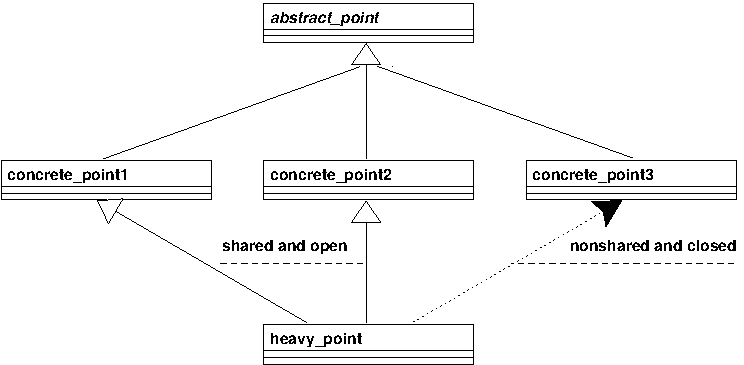
\includegraphics{heavy.pdf}}
\end{center}
\vspace{-33\in}
\caption{Diamond inheritance and beyond}
\label{F:heavy}
\end{figure*}



%%%%%%%%%%%%%%%%%%%%%%%%%%%%%%%%%%%%%%%%%%%%%%%%%%%%%%%%%%%%%%%%%%%%%%%%%%%%%
%%%%%%%%%%%%%%%%%%%%%%%%%%%%%%%%%%%%%%%%%%%%%%%%%%%%%%%%%%%%%%%%%%%%%%%%%%%%%
%%%%%%%%%%%%%%%%%%%%%%%%%%%%%%%%%%%%%%%%%%%%%%%%%%%%%%%%%%%%%%%%%%%%%%%%%%%%%



\subsection{Sophisticated inheritance boils down to record calculus}

In several OO languages, multiple inheritance is allowed. For
instance, in OCaml, the rules are as follows. Only the last definition
of a method is kept: the redefinition in a subclass of a method that
was visible in the parent class overrides the definition in the parent
class. Previous definitions of a method can be reused by binding the
related ancestor using a special \ldots @as@ \ldots notation.  The
bound name is said to be a pseudo value identifier that can only be
used to invoke an ancestor method. Other rules and notations exist for
Eiffel, C++, and so on.

In Haskell, we can handle more than plain multiple inheritance.
We are going to work through a scenario, where a class @heavy_point@
is constructed by inheritance from three different concrete subclasses
of @abstract_point@. The first two
concrete points will be shared in the resulting heavy point, because
we leave open the recursive knot. The third concrete point
does not participate in the open recursion; so it is not shared. See
Fig.~\ref{F:heavy} for an overview.

The object template for heavy points starts as follows:

\begin{code}
 heavy_point x_init color self =
  do
     super1 <- concrete_point1 x_init self
     super2 <- concrete_point2 x_init self
     super3 <- mfix (concrete_point3 x_init)
     ... -- to be continued
\end{code}

\noindent
That is, we bind all ancestor objects for subsequent reference. We
pass @self@ to the first two points, which participate in open
recursion, but we fix the third point in place. A heavy point carries
@print@ and @move@ methods that delegate corresponding messages to all
three points:

\begin{code}
     ... -- continued from above
     let myprint = do
                      putStr "super1: "; (super1 # print)
                      putStr "super2: "; (super2 # print)
                      putStr "super3: "; (super3 # print)
     let mymove  = ( \d -> do
                              super1 # move $ d
                              super2 # move $ d
                              super3 # move $ d )
     return 
       $    print  .=. myprint
      .*.   move   .=. mymove
      .*.   emptyRecord
     ... -- to be continued
\end{code}

\noindent
The three points, with all their many fields and methods, contribute
to the heavy point by means of left-biased union on records, which is
denoted by ``@.<++.@'' below:

\begin{code}
     ... -- continued from above
      .<++. super1
      .<++. super2
      .<++. super3
\end{code}

\noindent
(The routine definition of ``@.<++.@'' is given in App.~\ref{A:hLeftUnion}.)

\myskip

\noindent
It's time for a demo:

\begin{code}
 myDiamondOOP =
  do 
     p <- mfix (heavy_point 42 "blue")
     p # print -- All points still agree!
     p # move $ 2
     p # print -- The third point lacks behind!
\end{code}

\begin{code}
 ghci> myDiamondOOP
 super1: 42
 super2: 42
 super3: 42
 super1: 46
 super2: 46
 super3: 44
\end{code}



%%%%%%%%%%%%%%%%%%%%%%%%%%%%%%%%%%%%%%%%%%%%%%%%%%%%%%%%%%%%%%%%%%%%%%%%%%%%%
%%%%%%%%%%%%%%%%%%%%%%%%%%%%%%%%%%%%%%%%%%%%%%%%%%%%%%%%%%%%%%%%%%%%%%%%%%%%%
%%%%%%%%%%%%%%%%%%%%%%%%%%%%%%%%%%%%%%%%%%%%%%%%%%%%%%%%%%%%%%%%%%%%%%%%%%%%%



\subsection{No need for equi-recursive types}

We saw that our class constructor takes @self@ as an argument, and
returns the record, essentially @self'@, as the result. Our encoding
(for non-abstract classes) requires that @self@ and @self'@ have the
same slots -- but they do not have to be of the same type. This is how
we avoid recursive types. Later on, when we instantiate the class into
an object, we will apply @mfix@ operator -- that is, we will use value
recursion rather than the type recursion. Of course our technique
works if no method type involves the type of the self argument
(\emph{not} counting the implicit self). This is indeed the case in
most OO languages, where we must declare the type of the argument and
the result of a method, and that type must be a concrete type rather
than just `self'.  Functional objects obviously break this rule. We
have found a way to deal with functional objects while avoiding
recursive and existential types, but this topic is outside of the
scope of the present paper.



%%%%%%%%%%%%%%%%%%%%%%%%%%%%%%%%%%%%%%%%%%%%%%%%%%%%%%%%%%%%%%%%%%%%%%%%%%%%%
%%%%%%%%%%%%%%%%%%%%%%%%%%%%%%%%%%%%%%%%%%%%%%%%%%%%%%%%%%%%%%%%%%%%%%%%%%%%%
%%%%%%%%%%%%%%%%%%%%%%%%%%%%%%%%%%%%%%%%%%%%%%%%%%%%%%%%%%%%%%%%%%%%%%%%%%%%%

  


%%%%%%%%%%%%%%%%%%%%%%%%%%%%%%%%%%%%%%%%%%%%%%%%%%%%%%%%%%%%%%%%%%%%%%%%%%%%%
%%%%%%%%%%%%%%%%%%%%%%%%%%%%%%%%%%%%%%%%%%%%%%%%%%%%%%%%%%%%%%%%%%%%%%%%%%%%%
%%%%%%%%%%%%%%%%%%%%%%%%%%%%%%%%%%%%%%%%%%%%%%%%%%%%%%%%%%%%%%%%%%%%%%%%%%%%%
 

                                                                             
\begin{figure*}[t]
\begin{center}
\resizebox{.8\textwidth}{!}{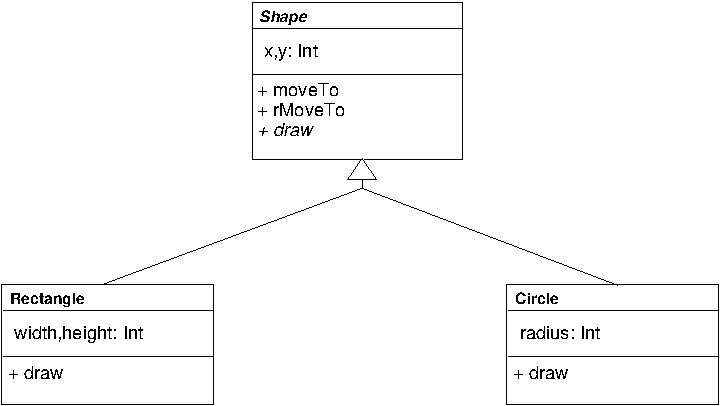
\includegraphics{shapes.pdf}}
\end{center}
\vspace{-33\in}
\caption{The `shapes' benchmark for subtype polymorphism}
\label{F:shapes}
\end{figure*}
                                                                             

 
%%%%%%%%%%%%%%%%%%%%%%%%%%%%%%%%%%%%%%%%%%%%%%%%%%%%%%%%%%%%%%%%%%%%%%%%%%%%%
%%%%%%%%%%%%%%%%%%%%%%%%%%%%%%%%%%%%%%%%%%%%%%%%%%%%%%%%%%%%%%%%%%%%%%%%%%%%%
%%%%%%%%%%%%%%%%%%%%%%%%%%%%%%%%%%%%%%%%%%%%%%%%%%%%%%%%%%%%%%%%%%%%%%%%%%%%%
 

 
\section{The Shapes benchmark}
\label{S:shapes}


Let us now explore the so-called `shapes benchmark'.\footnote{See the
multi-lingual collection `OO Example Code' by Jim Weirich at
\url{http://onestepback.org/articles/poly/}; see also an even heavier
collection `OO Shape Examples' by Chris Rathman at
\url{http://www.angelfire.com/tx4/cus/shapes/}.}  This benchmark (or
OO coding scenario) has a history in evaluating encodings of
subtype polymorphism. The classes that are involved in the
scenario are shown in Fig.~\ref{F:shapes}. There is an abstract class
(or an interface) @Shape@, and their are two subclasses @Rectangle@
and @Circle@. The coding scenario is the following: place different
shape object of different subclasses in a collection and iterate over
the collection to draw each shape object; the drawing
functionality varies per subclass.

We will show that the OOHaskell encoding pleasantly mimics the C++
encoding, while any remaining deviations are appreciated. We will also
discuss some variation points, once we have identified our prime
encoding. Finally, there are various possible encodings of the
scenario that do not deliver an image of Haskell as a true OO language
(including the one in Rathman's suite;
\url{http://www.angelfire.com/tx4/cus/shapes/haskell.html}). We do not
have space to discuss such non-OOHaskell encodings, but we refer to
this paper's source code distribution~\cite{OOHaskell} instead.



%%%%%%%%%%%%%%%%%%%%%%%%%%%%%%%%%%%%%%%%%%%%%%%%%%%%%%%%%%%%%%%%%%%%%%%%%%%%%
%%%%%%%%%%%%%%%%%%%%%%%%%%%%%%%%%%%%%%%%%%%%%%%%%%%%%%%%%%%%%%%%%%%%%%%%%%%%%
%%%%%%%%%%%%%%%%%%%%%%%%%%%%%%%%%%%%%%%%%%%%%%%%%%%%%%%%%%%%%%%%%%%%%%%%%%%%%



\subsection{The C++ reference solution}

We omit the code for the classes of shapes, rectangles and
circles. This is all trivial from a C++ perspective: we use a
pure virtual method for @draw@ in the class @Shape@, which is then
implemented differently in the classes @Rectangle@ and @Circle@.

Here is C++ code to set up an array of (two) shapes:

\begin{code}
   Shape *scribble[2];
   scribble[0] = new Rectangle(10, 20, 5, 6);
   scribble[1] = new Circle(15, 25, 8);
\end{code}

\noindent
We use an array rather than a collection type. We could employ a
collection type from C++'s Standard Template Library with similar
convenience. Here is a for-loop over the array in our C++ code:

\begin{code}
   for (int i = 0; i < 2; i++) {
      scribble[i]->draw();
      scribble[i]->rMoveTo(100, 100);
      scribble[i]->draw();
   }
\end{code}

\noindent
That is, we draw each element, move it relatively to its
origin, and draw it again. If the @draw@ method prints
`progress messages' about what is being drawn, we may see the
following output:

\begin{code}
 Drawing a Rectangle at:(10,20), width 5, height 6
 Drawing a Rectangle at:(110,120), width 5, height 6
 Drawing a Circle at:(15,25), radius 8
 Drawing a Circle at:(115,125), radius 8
\end{code}

\noindent
(Any OO language with parametric polymorphism, or at least polymorphic
arrays, should allow similarly concise code. In a typed language
without parametric polymorphism, we would need to bother about unsafe
down-casts when processing the aggregated objects. Likewise, untyped
languages would risk `message-not-understood' errors.)



%%%%%%%%%%%%%%%%%%%%%%%%%%%%%%%%%%%%%%%%%%%%%%%%%%%%%%%%%%%%%%%%%%%%%%%%%%%%%
%%%%%%%%%%%%%%%%%%%%%%%%%%%%%%%%%%%%%%%%%%%%%%%%%%%%%%%%%%%%%%%%%%%%%%%%%%%%%
%%%%%%%%%%%%%%%%%%%%%%%%%%%%%%%%%%%%%%%%%%%%%%%%%%%%%%%%%%%%%%%%%%%%%%%%%%%%%



\subsection{The OOHaskell transcription}

We also omit the Haskell values for the involved classes since we have
exercised pure virtual methods in Sec.~\ref{S:self}. We only
transcribe the collection code. We start a monadic @do@ sequence to
construct two shape objects~---~just as above:

\begin{code}
 myShapesOOP =
    do
       s1 <- mfix (rectangle (10::Int) (20::Int) 5 6)
       s2 <- mfix (circle (15::Int) 25 8)
       -- to be continued
\end{code}

\noindent
What's different? We use @mfix@ in place of @new@. We use curried
functions instead of C++'s comma notation.  We note that some
constructor arguments are annotated by the @Int@ type because we
preferred to eliminate the implicit polymorphism at this stage.

We continue the monadic @do@ sequence by building an `array' of
shapes:

\begin{code}
       let scribble :: [Shape Int]
           scribble = [narrow s1, narrow s2]
\end{code}

\noindent
In fact, we use a plain Haskell list. The type annotation for the
@scribble@ binding corresponds to the typed variable declaration in
the C++ code. However, the Haskell list construction differs from the
the C++ array construction as follows. In Haskell, we use an
explicit coercion operation, @narrow@ to prepare each shape object for
insertion into the homogeneous list. By contrast, such casting is
\emph{implicit} in the C++ code.

Regarding the class type @Shape@, we note that we have not used
\emph{any} explicit class types in the preceding sections. Mostly, we
do not need them because Haskell's type inference works
fine. (Programmers of C++ and of other mainstream languages have
the habit of writing down types for almost everything.) For the
purpose of \emph{casting}, we require such explicit types in
OOHaskell. They are necessary for steering explicit casting in the
view of programs that otherwise lack pervasive type annotations: So
here is the record type for @Shape@ objects:

\begin{code}
 type Shape a = Record (  (Proxy GetX    , IO a)
                      :*: (Proxy GetY    , IO a)
                      :*: (Proxy SetX    , a -> IO ())
                      :*: (Proxy SetY    , a -> IO ())
                      :*: (Proxy MoveTo  , a -> a -> IO ())
                      :*: (Proxy RMoveTo , a -> a -> IO ())
                      :*: (Proxy Draw    , IO ())
                      :*: HNil )
\end{code}

We finish up the monadic @do@ sequence by iterating over scribble:

\begin{code}
       mapM_ (\shape -> do
                           shape # draw
                           (shape # rMoveTo) 100 100
                           shape # draw)
             scribble
\end{code}

\noindent
Here we use the monadic @mapM_@ operation which only cares about the
effects of the monadic steps, throwing away results. This is really
the Haskell way of iterating over a list with effectful
functions~---~as the counterpart of the for-loop in the C++ code.



%%%%%%%%%%%%%%%%%%%%%%%%%%%%%%%%%%%%%%%%%%%%%%%%%%%%%%%%%%%%%%%%%%%%%%%%%%%%%
%%%%%%%%%%%%%%%%%%%%%%%%%%%%%%%%%%%%%%%%%%%%%%%%%%%%%%%%%%%%%%%%%%%%%%%%%%%%%
%%%%%%%%%%%%%%%%%%%%%%%%%%%%%%%%%%%%%%%%%%%%%%%%%%%%%%%%%%%%%%%%%%%%%%%%%%%%%



\subsection{Narrowing vs.\ heterogeneity vs.\ existentials}

We have employed narrowing to coerce all objects to a common
interface, in fact, to the \emph{same} record type. One might wonder
whether these coercions can be avoided altogether, or whether the
explicit conversions can also be made implicit even in OOHaskell. We
will discuss two techniques, but the conclusion will be that narrowing
is to be preferred.

The first technique is to collect the shape objects, as is, in a
\emph{heterogeneous} list rather than a homogeneous array or list. We
cannot construct such a list with the normal, polymorphic list datatype
constructor, but the \HList\ library comes again to our rescue. 
The scribble construction can now be performed without any
narrowing:

\begin{code}
       let scribble = s1 `HCons` (s2 `HCons` HNil)
\end{code}

\noindent
We cannot use ordinary list-processing function anymore, but the
\HList\ library mimics the normal list-processing API for @HList@s. So
there is also a heterogeneous variation on @mapM_@, namely @hMapM_@,
to be invoked as follows:

\begin{Verbatim}[fontsize=\small,commandchars=\\\{\}]
       hMapM_ (\undefined::FunOnShape) scribble
\end{Verbatim}

\noindent
The first argument of @hMapM_@ is not a function but rather a
\emph{type code}. This is necessary for technical reasons related to
the combination of rank-n polymorphism and ad-hoc
polymorphism.\footnote{A heterogeneous map function can encounter
entities of different types. Hence, its argument function must be
polymorphic on its own (which is different from the normal map
function). The argument function typically uses type classes (say,
ad-hoc polymorphism) to process the entities of different types. The
trouble is that the map function cannot possibly anticipate all the
constraints required by its argument function.  The type-code
technique moves the constraints from the type of the heterogeneous map
function to the interpretation site of the type codes.} The meaning of
each type code must be defined by a dedicated instance of an @Apply@
class for function application. Here is the declaration of the type
code @FunOnShape@ complete with its meaning:

\begin{code}
 data FunOnShape -- a type code only!
\end{code}

\begin{code}
instance ( HasField (Proxy Draw) r (IO ())
         , HasField (Proxy RMoveTo) r (Int -> Int -> IO ())
         )
      => Apply FunOnShape r (IO ())
  where
    apply _ x = do
                   x # draw
                   (x # rMoveTo) 100 100
                   x # draw
\end{code}

\noindent
The @Apply@ instance manifests encoding efforts that we didn't face
for the narrowing-based encoding. Now we have to list the
\emph{method-access constraints} (for ``\#'', i.e., @HasField@) in the
@Apply@ instance. Haskell's type-class system requires us to provide
proper bounds for the instance. One might argue that the form of these
constraints strongly resembles the method types listed in the class
type @Shape@. So one might wonder whether we can somehow use the full
class type in order to constrain the instance.  Haskell won't let us
do that in any reasonable way. (Constraints are not first-class
citizens in Haskell; we can't compute them from types or type
proxies~---~unless we were willing to rely on heavy encoding or
advanced syntactic sugar.) So we are doomed to manually infer such
method-access constraints for each such piece of polymorphic code.

The second technique for avoiding narrowing relies on placing shape
objects in \emph{existentially quantified envelopes}: we do not
coerce, but we wrap:

\begin{code}
       let scribble = [ WrapShape s1 , WrapShape s2 ]
\end{code}

\noindent
The declaration of the @WrapShape@ type depends on the function that
we want to apply to the opaque data. In our case, we can use the
normal @mapM_@ function again; we only need to unwrap the @WrapShape@
constructor prior to method invocations:

\begin{code}
       mapM_ ( \(WrapShape shape) -> do
                  shape # draw
                  (shape # rMoveTo) 100 100
                  shape # draw )
             scribble
\end{code}

\noindent
These operations have to be anticipated in the type bound for
@WrapShape@:

\begin{Verbatim}[fontsize=\small,commandchars=\\\{\}]
 data WrapShape =
  \Forall x. ( HasField (Proxy Draw) x (IO ())
       , HasField (Proxy RMoveTo) x (Int -> Int -> IO ())
       ) => WrapShape x
\end{Verbatim}

\noindent
It becomes evident that this result agrees with the heterogeneity
technique in terms of encoding efforts. In both cases, we need to
identify type-class constraints that correspond to the (potentially)
polymorphic method invocations.

Consequently, the narrowing technique is to be preferred.  We
\emph{could} hide narrowing by eschewing free-wheeling functional
programming and type inference. The required style and API would then
account for hidden narrowing. We do not favour such an approach for
various reasons. Abandoning type inference is in conflict with Haskell
native style.  Making casts implicit introduces the risk that the
programmer can accidentally pass an object of the wrong type.  Making
cast implicit hides the costs that come with casts; we prefer to see
the need for coercions clearly. (In fact, in the presence of multiple
inheritance of classes or interfaces, the implicit cast is absolutely
nontrivial, either for the compiler, or for the run-time system, or
both.)



%%%%%%%%%%%%%%%%%%%%%%%%%%%%%%%%%%%%%%%%%%%%%%%%%%%%%%%%%%%%%%%%%%%%%%%%%%%%%
%%%%%%%%%%%%%%%%%%%%%%%%%%%%%%%%%%%%%%%%%%%%%%%%%%%%%%%%%%%%%%%%%%%%%%%%%%%%%
%%%%%%%%%%%%%%%%%%%%%%%%%%%%%%%%%%%%%%%%%%%%%%%%%%%%%%%%%%%%%%%%%%%%%%%%%%%%%



 
%%%%%%%%%%%%%%%%%%%%%%%%%%%%%%%%%%%%%%%%%%%%%%%%%%%%%%%%%%%%%%%%%%%%%%%%%%%%%
%%%%%%%%%%%%%%%%%%%%%%%%%%%%%%%%%%%%%%%%%%%%%%%%%%%%%%%%%%%%%%%%%%%%%%%%%%%%%
%%%%%%%%%%%%%%%%%%%%%%%%%%%%%%%%%%%%%%%%%%%%%%%%%%%%%%%%%%%%%%%%%%%%%%%%%%%%%
 

 
\section{Final discussion}
\label{S:disc}

We have described an OOP system for Haskell that supports stateful
objects, inheritance and subtype polymorphism. The Shapes Benchmark
demonstrated that our encoding is very close to the textbook OO code
(usually given in C++ or Java tutorials), with pleasant
deviations. The re-implementation of examples from the OCaml object
tutorial demonstrated the faithfulness of our realisation of
objects. (We have opted for OCaml because it is a leading object
system in a functional setting.) We have implemented parameterised
classes, constructor methods, abstract classes, pure virtual methods,
single and multiple inheritance with flexible rules of sharing or
separation of superclasses. Major byproducts are these: extensive type
inference, first-class classes, sharing of the code of methods among
even non-related classes, implicit polymorphism of classes, fully
static type checking.

We have clarified the relation between subtyping and type-class based
polymorphism: the latter can encode the former. We have implemented
OOHaskell with the existing Haskell implementation (GHC), requiring no
extra extensions beyond the commonly implemented ones: multi-parameter
type classes with functional dependencies. It is quite pleasant that
the existing OOHaskell code does not seem to be a burden to
write~---~even in the absence of any syntactic sugar.  Once we
consider open recursion in our setup, it turns out that the object
constructor (i.e., `new') is merely the monadic fix-point operation
(i.e., `mfix'). Just as people have known all the time~---~OO and
recursion are intertwined.

There exists a large body of literature,
e.g.,~\cite{Poll97,AC96,Ohori95,Remy94a,PT94,BM92}. Most often
discussed are pure functional objects. Most often the type systems of
object models are variants of system $F_{\leq}$ (polymorphic
lambda-calculus plus subtyping). Most often objects with open
recursion are represented either with recursive types, or with
existentially quantified types. In the present paper we demonstrated
the encoding of imperative objects with inheritance and polymorphism
in Haskell~---~that is, polymorphic lambda-calculus plus
multi-parameter type classes with functional dependencies. Unlike
$F_{\leq}$, there is no built-in subtyping relation. It is remarkable
that our encoding of imperative objects avoids both recursive types
and existentially quantified types. A particularly interesting case
are functional objects, which seem to require recursive or
existentially-quantified types. Functional objects and preservation of
type inference is to be discussed in a forthcoming paper.  Our current
implementation has strong similarities with prototype-based systems
(such as Self~\cite{Self}) in that mutable fields and method
`pointers' are a part of the same record. This does not have to be the
case~---~and in fact, in the forthcoming paper on pure-functional
objects we separate the two tables (in the manner similar to object
realisations in C++ or Java).

There are some further idioms that complement OOHaskell as a faithful
OOP system.  For instance, we need to take measures to do
instantiation checking for classes at declaration time. Otherwise some
type errors would go unnoticed until the first attempt to programme an
instantiation. We can also model various forms of private and
protected methods and other access modifiers. We can clone objects, we
can let methods return `self', we can operate in the ST monad rather
than the IO monad. The article comes with an extensive collection of
source code~\cite{OOHaskell}, where these and other issues are
covered. The source code also illustrates some cases of depth
subtyping~\cite{Poll97} and statically safe argument
covariance. However, the extent and limitations of our handling of
depth subtyping remains the subject of ongoing research.

We are currently working on some elaborations and advanced topics.
Simple syntactic sugar would make OOP more convenient in Haskell.
Extra effort is needed to provide OOP-like error messages.  This is a
sticking issue that requires major effort, but there is a line of
research being carried out by Sulzmann and others~\cite{SSW04}. A
non-trivial case study is required to demonstrate the scalability of
the approach. The mere compilation time of OOHaskell programs and
their runtime efficiency is challenged by the huge dictionaries that
are implied by our type-class-based approach.  It seems that some
dedicated optimisations will be needed in order to handle the
\HList/OOHaskell style of programming efficiently. An interesting
advanced topic is reflective programming. A simple form of reflection
is readily provided in terms of the type-level encoding of
records. One can iterate over records and their components in a
generic fashion. Other forms of reflection, such as iteration over the
object pool, as needed for dynamic aspect-oriented programming,
requires further effort. Another challenge is to capture reusable
solutions for design problems (as part of design patterns) in Haskell.



%%%%%%%%%%%%%%%%%%%%%%%%%%%%%%%%%%%%%%%%%%%%%%%%%%%%%%%%%%%%%%%%%%%%%%%%%%%%%
%%%%%%%%%%%%%%%%%%%%%%%%%%%%%%%%%%%%%%%%%%%%%%%%%%%%%%%%%%%%%%%%%%%%%%%%%%%%%
%%%%%%%%%%%%%%%%%%%%%%%%%%%%%%%%%%%%%%%%%%%%%%%%%%%%%%%%%%%%%%%%%%%%%%%%%%%%%




%%%%%%%%%%%%%%%%%%%%%%%%%%%%%%%%%%%%%%%%%%%%%%%%%%%%%%%%%%%%%%%%%%%%%%%%%%%%%
%%%%%%%%%%%%%%%%%%%%%%%%%%%%%%%%%%%%%%%%%%%%%%%%%%%%%%%%%%%%%%%%%%%%%%%%%%%%%
%%%%%%%%%%%%%%%%%%%%%%%%%%%%%%%%%%%%%%%%%%%%%%%%%%%%%%%%%%%%%%%%%%%%%%%%%%%%%



{\small 

\subsubsection*{Acknowledgements}
 
We thank Chung-chieh Shan for very helpful discussions. The second
author presented this work at an earlier stage at the WG2.8 meeting
(Functional Programming) in November 2004 at West Point. We are
grateful for feedback at this meeting. We also appreciated feedback from
Robin Green, Bryn Keller, Chris Rath and several other participants
in mailing list or email discussions. 

}



%%%%%%%%%%%%%%%%%%%%%%%%%%%%%%%%%%%%%%%%%%%%%%%%%%%%%%%%%%%%%%%%%%%%%%%%%%%%%
%%%%%%%%%%%%%%%%%%%%%%%%%%%%%%%%%%%%%%%%%%%%%%%%%%%%%%%%%%%%%%%%%%%%%%%%%%%%%
%%%%%%%%%%%%%%%%%%%%%%%%%%%%%%%%%%%%%%%%%%%%%%%%%%%%%%%%%%%%%%%%%%%%%%%%%%%%%



\bibliographystyle{abbrv}
\bibliography{paper}



%%%%%%%%%%%%%%%%%%%%%%%%%%%%%%%%%%%%%%%%%%%%%%%%%%%%%%%%%%%%%%%%%%%%%%%%%%%%%
%%%%%%%%%%%%%%%%%%%%%%%%%%%%%%%%%%%%%%%%%%%%%%%%%%%%%%%%%%%%%%%%%%%%%%%%%%%%%
%%%%%%%%%%%%%%%%%%%%%%%%%%%%%%%%%%%%%%%%%%%%%%%%%%%%%%%%%%%%%%%%%%%%%%%%%%%%%



\renewcommand{\mysize}{\footnotesize}



\medskip

\section{Type extension by polymorphic data tails}

Each OO class amounts to a normal Haskell record type, which has an
extension point for subclassing so to say. This extension point is
necessarily a component of a parametrically polymorphic type that is
exposed as a type parameter of the record type. When we transcribe a
subclass, we simply \emph{further} instantiate the record type for its
base class with its own associated record type. Methods are simply
defined for the record type that is sufficiently instantiated to allow
access to the relevant components (at some level), but not more
instantiated than necessary for the sake of subtyping
polymorphism. Virtual methods need to be defined in dedicated Haskell
type classes.

There are some possible variations on this theme.


%%%%%%%%%%%%%%%%%%%%%%%%%%%%%%%%%%%%%%%%%%%%%%%%%%%%%%%%%%%%%%%%%%%%%%%%%%%%%
%%%%%%%%%%%%%%%%%%%%%%%%%%%%%%%%%%%%%%%%%%%%%%%%%%%%%%%%%%%%%%%%%%%%%%%%%%%%%
%%%%%%%%%%%%%%%%%%%%%%%%%%%%%%%%%%%%%%%%%%%%%%%%%%%%%%%%%%%%%%%%%%%%%%%%%%%%%



\medskip

\subsection{The Shape class}

\begin{code}
-- Mutable data of extensible shapes
data Shape w =
     Shape { getX     :: Int
           , getY     :: Int
           , shapeExt :: w
           }

-- Constructor for shapes
shape x y w = Shape { getX = x
                    , getY = y
                    , shapeExt = w }

-- Setters
setX :: Int -> Shape w -> Shape w
setX i s = s { getX = i }

setY :: Int -> Shape w -> Shape w
setY i s = s { getY = i }

-- Move methods on shapes
moveTo :: Int -> Int -> Shape w -> Shape w
moveTo x y = setY y . setX x 

rMoveTo :: Int -> Int -> Shape w -> Shape w
rMoveTo deltax deltay s = moveTo x y s
 where
  x = getX s + deltax
  y = getY s + deltay

-- The abstract method for drawing shapes
class Draw w
 where
  draw :: Shape w -> IO()
\end{code}



%%%%%%%%%%%%%%%%%%%%%%%%%%%%%%%%%%%%%%%%%%%%%%%%%%%%%%%%%%%%%%%%%%%%%%%%%%%%%
%%%%%%%%%%%%%%%%%%%%%%%%%%%%%%%%%%%%%%%%%%%%%%%%%%%%%%%%%%%%%%%%%%%%%%%%%%%%%
%%%%%%%%%%%%%%%%%%%%%%%%%%%%%%%%%%%%%%%%%%%%%%%%%%%%%%%%%%%%%%%%%%%%%%%%%%%%%



\medskip

\subsection{The Circle class}

\begin{code}
-- The delta of circles
data Circlish w =
     Circlish { getRadius :: Int 
              , circleExt :: w
              }

-- An extension of Shape
type Circle w = Shape (Circlish w)

-- A "closed" constructor
circle x y r
 = shape x y $ Circlish { getRadius = r
                        , circleExt = () }

-- Setter
setRadius :: Int -> Circle w -> Circle w
setRadius i s
 = s { shapeExt = (shapeExt s) { getRadius = i } }

-- Implement abstract draw method
instance Draw (Circlish w)
 where
  draw s =  putStrLn ("Drawing a Circle at:("
         ++ (show (getX s))
         ++ ","
         ++ (show (getY s))
         ++ "), radius "
         ++ (show (getRadius (shapeExt s))))
\end{code}



%%%%%%%%%%%%%%%%%%%%%%%%%%%%%%%%%%%%%%%%%%%%%%%%%%%%%%%%%%%%%%%%%%%%%%%%%%%%%
%%%%%%%%%%%%%%%%%%%%%%%%%%%%%%%%%%%%%%%%%%%%%%%%%%%%%%%%%%%%%%%%%%%%%%%%%%%%%
%%%%%%%%%%%%%%%%%%%%%%%%%%%%%%%%%%%%%%%%%%%%%%%%%%%%%%%%%%%%%%%%%%%%%%%%%%%%%



\medskip

\subsection{The Rectangle class}

Omitted. Very much like the Circle class.



%%%%%%%%%%%%%%%%%%%%%%%%%%%%%%%%%%%%%%%%%%%%%%%%%%%%%%%%%%%%%%%%%%%%%%%%%%%%%
%%%%%%%%%%%%%%%%%%%%%%%%%%%%%%%%%%%%%%%%%%%%%%%%%%%%%%%%%%%%%%%%%%%%%%%%%%%%%
%%%%%%%%%%%%%%%%%%%%%%%%%%%%%%%%%%%%%%%%%%%%%%%%%%%%%%%%%%%%%%%%%%%%%%%%%%%%%



\medskip

\subsection{Scribble processing}

\begin{code}
-- Existential envelope for `drawables'
data Drawable = forall a. Draw a
  => Drawable (Shape a)

-- Weirich's / Rathman's test case
main =
      do
         -- Handle the shapes polymorphically
         mapM_ ( \(Drawable x) -> 
                   do
                      draw x
                      draw (rMoveTo 100 100 x))
               scribble

         -- Handle rectangle-specific instance
         draw $ setWidth 30 arectangle

      where
         -- Create some shape instances
         scribble = [
            Drawable (rectangle 10 20 5 6),
            Drawable (circle 15 25 8)]

         -- Create a rectangle instance
         arectangle = (rectangle 0 0 15 15)
\end{code}



%%%%%%%%%%%%%%%%%%%%%%%%%%%%%%%%%%%%%%%%%%%%%%%%%%%%%%%%%%%%%%%%%%%%%%%%%%%%%
%%%%%%%%%%%%%%%%%%%%%%%%%%%%%%%%%%%%%%%%%%%%%%%%%%%%%%%%%%%%%%%%%%%%%%%%%%%%%
%%%%%%%%%%%%%%%%%%%%%%%%%%%%%%%%%%%%%%%%%%%%%%%%%%%%%%%%%%%%%%%%%%%%%%%%%%%%%



\medskip

\section{Type extension by record composition}


As an aside, one may actually argue that this approach is less about
inheritance; it is perhaps closer to delegation. Each OO class
amounts to a normal Haskell record type, where a derived class
aggregates a component for its ancestor class. When a method is
introduced at some level in the inheritance hierarchy we just define
it for that very type. We can represent the inheritance hierarchy by
means of a dedicated subtyping class which also allows us to lift
methods from the introducing class to subclasses. Virtual methods need
to be defined in dedicated Haskell type classes.



There are some possible variations on this theme.



%%%%%%%%%%%%%%%%%%%%%%%%%%%%%%%%%%%%%%%%%%%%%%%%%%%%%%%%%%%%%%%%%%%%%%%%%%%%%
%%%%%%%%%%%%%%%%%%%%%%%%%%%%%%%%%%%%%%%%%%%%%%%%%%%%%%%%%%%%%%%%%%%%%%%%%%%%%
%%%%%%%%%%%%%%%%%%%%%%%%%%%%%%%%%%%%%%%%%%%%%%%%%%%%%%%%%%%%%%%%%%%%%%%%%%%%%



\medskip

\subsection{The concept of subtyping} 

We keep track of the OO inheritance hierarchy by means of a dedicated
Haskell class @Subtype@. This class hosts two methods for applying
observers vs.\ mutators to objects. This is an essential convenience
layer for defining accessors (getters/setters) on object types such
that they also work on derived types.

The use of a two-parameter type-class is not really essential.  In
Haskell 98, we would simply specialise this type-class per OO class.
MP Jones and SP Jones adopt this idea in "OO style overloading for
Haskell", even though they do not consider state.

Note that there is a reflexive instance for subtyping. It would be
possible to eliminate the use of a generic instance.  That is we could
use specific instances per actual OO class.  Transitivity (along
subtyping chains) is not so easily taken care of. For each new type,
we need to provide instances for all ancestors.


\begin{code}
infix 7 .?. -- observation
infix 7 .!. -- mutation

class Subtype a b where
 (.?.) :: (b -> r) -> a -> r
 (.!.) :: (b -> b) -> a -> a

instance Subtype a a where
 (.?.) = id
 (.!.) = id
\end{code}



%%%%%%%%%%%%%%%%%%%%%%%%%%%%%%%%%%%%%%%%%%%%%%%%%%%%%%%%%%%%%%%%%%%%%%%%%%%%%
%%%%%%%%%%%%%%%%%%%%%%%%%%%%%%%%%%%%%%%%%%%%%%%%%%%%%%%%%%%%%%%%%%%%%%%%%%%%%
%%%%%%%%%%%%%%%%%%%%%%%%%%%%%%%%%%%%%%%%%%%%%%%%%%%%%%%%%%%%%%%%%%%%%%%%%%%%%



\medskip

\subsection{The Shape class}

\begin{code}
-- Mutable data of shapes
data Shape =
     Shape { getX    :: Int
           , getY    :: Int
           }

-- Constructor for shapes
shape x y = Shape { getX = x
                  , getY = y }

-- Setters
setX :: Subtype a Shape => Int -> a -> a
setX i = (.!.) (\s -> s { getX = i} )

setY :: Subtype a Shape => Int -> a -> a
setY i = (.!.) (\s -> s { getY = i} )

-- Move methods on shapes
moveTo :: Subtype a Shape => Int -> Int -> a -> a
moveTo x y = setY y . setX x 

rMoveTo :: Subtype a Shape => Int -> Int -> a -> a
rMoveTo deltax deltay a = moveTo x y a
 where
  x = getX .?. a + deltax
  y = getY .?. a + deltay

-- The abstract method for drawing shapes
class Subtype a Shape => Draw a
 where
  draw :: a -> IO()
\end{code}



%%%%%%%%%%%%%%%%%%%%%%%%%%%%%%%%%%%%%%%%%%%%%%%%%%%%%%%%%%%%%%%%%%%%%%%%%%%%%
%%%%%%%%%%%%%%%%%%%%%%%%%%%%%%%%%%%%%%%%%%%%%%%%%%%%%%%%%%%%%%%%%%%%%%%%%%%%%
%%%%%%%%%%%%%%%%%%%%%%%%%%%%%%%%%%%%%%%%%%%%%%%%%%%%%%%%%%%%%%%%%%%%%%%%%%%%%



\medskip

\subsection{The Circle class}

\begin{code}
-- An extension of Shape
data Circle =
     Circle { circle2shape :: Shape
            , getRadius :: Int }

-- Constructor
circle x y r
 = Circle { circle2shape = shape x y
          , getRadius = r }

-- Instantiate the subtyping relation
instance Subtype Circle Shape
 where
  f .?. a = f $ circle2shape $ a
  f .!. a = a { circle2shape = f $ circle2shape a }

-- Setter
setRadius :: Subtype a Circle => Int -> a -> a
setRadius i = (.!.) (\s -> s { getRadius = i} )

-- Implement abstract draw method
instance Draw Circle
 where
  draw a =  putStrLn ("Drawing a Circle at:("
         ++ (show (getX .?. a))
         ++ ","
         ++ (show (getY .?. a))
         ++ "), radius "
         ++ (show (getRadius .?. a)))
\end{code}



%%%%%%%%%%%%%%%%%%%%%%%%%%%%%%%%%%%%%%%%%%%%%%%%%%%%%%%%%%%%%%%%%%%%%%%%%%%%%
%%%%%%%%%%%%%%%%%%%%%%%%%%%%%%%%%%%%%%%%%%%%%%%%%%%%%%%%%%%%%%%%%%%%%%%%%%%%%
%%%%%%%%%%%%%%%%%%%%%%%%%%%%%%%%%%%%%%%%%%%%%%%%%%%%%%%%%%%%%%%%%%%%%%%%%%%%%



\medskip

\subsection{The Rectangle class}

Omitted. Very much like the Circle class.



%%%%%%%%%%%%%%%%%%%%%%%%%%%%%%%%%%%%%%%%%%%%%%%%%%%%%%%%%%%%%%%%%%%%%%%%%%%%%
%%%%%%%%%%%%%%%%%%%%%%%%%%%%%%%%%%%%%%%%%%%%%%%%%%%%%%%%%%%%%%%%%%%%%%%%%%%%%
%%%%%%%%%%%%%%%%%%%%%%%%%%%%%%%%%%%%%%%%%%%%%%%%%%%%%%%%%%%%%%%%%%%%%%%%%%%%%



\medskip

\subsection{Scribble processing}

Compared to the "type extension by polymorphic record tails" approach,
the only difference is that we do not necessarily face Shape records
but potentially also records that contain Shape records. The only
place where this detail matters is in the definition of the
existential envelope.

\begin{code}
-- Existential envelope for `drawables'
data Drawable = forall a. Draw a
  => Drawable a
\end{code}




%%%%%%%%%%%%%%%%%%%%%%%%%%%%%%%%%%%%%%%%%%%%%%%%%%%%%%%%%%%%%%%%%%%%%%%%%%%%%
%%%%%%%%%%%%%%%%%%%%%%%%%%%%%%%%%%%%%%%%%%%%%%%%%%%%%%%%%%%%%%%%%%%%%%%%%%%%%
%%%%%%%%%%%%%%%%%%%%%%%%%%%%%%%%%%%%%%%%%%%%%%%%%%%%%%%%%%%%%%%%%%%%%%%%%%%%%



\end{document}
